\documentclass[notitlepage,aps,prd,nofootinbib]{revtex4-1}
  
\newcommand{\figures}{../outputs/plots}
\newcommand{\includedir}{../latex_files}

%%%%%%%%%%%%%%%%%%%%%%%%%%%%%%%%%%%%%%%%%%%%%%%%%%
% usepackages
\usepackage{amsmath,amssymb,bbm}
\usepackage{graphicx}
\usepackage[protrusion=true,expansion=true]{microtype} % make text fow nice...
\usepackage{verbatim} % verbatim text and comment environment
\usepackage{lmodern} % allowing font sizes at arbitrary sizes
\usepackage{appendix}
\usepackage[free-standing-units]{siunitx} % units package, see https://www.ctan.org/pkg/siunitx
\usepackage[absolute,overlay]{textpos} % for textblock* absolute positioning 
\TPGrid{100}{100} % make our textpos grid 100 by 100 for easy positioning 
% \TPGrid[20mm,20mm]{100}{100} % default mm grid
%\usepackage[texcoord,grid,gridunit=mm,gridcolor=red!10,subgridcolor=green!10]{eso-pic} % layout grid, mm
%\usepackage{tcolorbox}
%\usepackage{enumitem}
%\usepackage{fancyvrb}
%\usepackage{ulem}
%\usepackage{listings}
\usepackage{overpic}
\usepackage[section]{placeins}

%%%%%%%%%%%%%%%%%%%%%%%%%%%%%%%%%%%%%%%%%%%%%%%%%%
% Include commands, style, colors, and abbreviations
% Load colors for everything!
\makeatletter
\@ifpackageloaded{xcolor}
 {% true
 }{% false
   % \usepackage[usenames,dvipsnames,svgnames,table]{xcolor}
   \usepackage[usenames]{xcolor}
 }
\makeatother

% Colors from https://styleguide.duke.edu/color-palette/

% These are the official colors, and they cannot be modified by the program (ie changing the opacity or saturation)
\definecolor{Duke Blue}{HTML}{001A57}
\definecolor{Blue Devil Blue}{HTML}{0736A4}

% These are the official recommendations for colors to go with the two official Duke colors. PMS is the Pantone Matching system index, so you can search the color to see what it should look like
\definecolor{PMS Black 3}{HTML}{262626}
\definecolor{PMS Cool Gray 11}{HTML}{666666}
\definecolor{PMS Cool Gray 7}{HTML}{B5B5B5}
\definecolor{PMS Cool Gray 3}{HTML}{E5E5E5}
\definecolor{Light Gray}{HTML}{F5F5F5}

% Blues
\definecolor{PMS 294}{HTML}{003366}
\definecolor{PMS 3015}{HTML}{235F9C}
\definecolor{PMS 3005}{HTML}{0680CD}

% Oranges
\definecolor{PMS 166}{HTML}{D75404}
\definecolor{PMS 1805}{HTML}{CC3300}
% \definecolor{PMS 157}{HTML}{F09905}

% Other
\definecolor{PMS 392}{HTML}{728302} % dark green
\definecolor{PMS 390}{HTML}{A1B70D} % light green
\definecolor{PMS 123}{HTML}{FFD960} % light yellow
\definecolor{PMS 2617}{HTML}{993399} % nice violet

% Define colors for Zeppenfeld_hadronization diagram
% \definecolor{zorange}{HTML}{ffd700}
% \definecolor{zpink}{HTML}{ff789e}
% \definecolor{zbrown}{HTML}{a14001}
% \definecolor{zpurple}{HTML}{d100d1}
% \definecolor{zgrey}{HTML}{e6e6e6}

% Define colors for hadronic shower diagram
% \definecolor{hsblue}{HTML}{0e2fff}
% \definecolor{hsred}{HTML}{ff2900}
% \definecolor{hsgreen}{HTML}{009d00}
% \definecolor{hsblack}{HTML}{000000}


% \definecolor{PMS }{HTML}{} % 



\usepackage{tikz}
\usepackage{adjustbox}
% \usepackage{graphicx}

% \includetikz{boxwidth}{tikzname}

\newcommand{\includetikz}[2]{%

% \framebox{ % show the frame around our box, for debugging spacing issues

    \resizebox{#1}{!}{%
      \centering
      \begin{tikzpicture}[remember picture]%
        \pic[anchor=center,draw,scale=1]{#2};%
      \end{tikzpicture}%
    } % end resizebox

%  } % end of framebox

} % end of newcommand

 % my general commands
%%%%%%%%%%%%%%%%%%%%%%%%%%%%%%%%%%%%%%%%%%%%%%%%%%%%%%%%%%%%%%%%%%%%%%%%%%%%%%%%%%%%%%%%%%%%%%%%%%%%
% Turn off revtex4-1 meaningless float warnings
\usepackage{silence} \WarningFilter{revtex4-1}{Repair the float}

%%%%%%%%%%%%%%%%%%%%%%%%%%%%%%%%%%%%%%%%%%%%%%%%%%%%%%%%%%%%%%%%%%%%%%%%%%%%%%%%%%%%%%%%%%%%%%%%%%%%
% Make the revtex4-1 date not have annoying parentheses any more
\usepackage{etoolbox}
\makeatletter
% \frontmatter@RRAP@format is responsible for the parentheses
\patchcmd{\frontmatter@RRAP@format}{(}{}{}{}
\patchcmd{\frontmatter@RRAP@format}{)}{}{}{}
\renewcommand\Dated@name{}
\makeatother

\usepackage[top=1in, bottom=1.25in, left=1.25in, right=1.25in]{geometry}

%%%%%%%%%%%%%%%%%%%%%%%%%%%%%%%%%%%%%%%%%%%%%%%%%%%%%%%%%%%%%%%%%%%%%%%%%%%%%%%%%%%%%%%%%%%%%%%%%%%%
% citation and href links auto-color
% \let\oldcite=\cite                                                              
% \renewcommand{\cite}[1]{\textcolor{Blue Devil Blue}{\oldcite{#1}}}

% \let\oldhref=\href                                                              
% \renewcommand{\href}[2]{\textcolor{Blue Devil Blue}{\oldhref{#1}{#2}}}

% \let\oldurl=\url                                                              
% \renewcommand{\url}[2]{\textcolor{Blue Devil Blue}{\oldurl{#1}{#2}}}



%%%%%%%%%%%%%%%%%%%%%%%%%%%%%%%%%%%%%%%%%%%%%%%%%%%%%%%%%%%%%%%%%%%%%%%%%%%%%%%%%%%%%%%%%%%%%%%%%%%%
% customized title page

%\makeatletter
%\let\insertadvisor\relax
%\newcommand\advisortitle{Advisor}
%\mode<all>
%{
%  \newcommand\advisor[1]{\def\insertadvisor{#1}}
%}
%
%
%\newtoggle{atlasLogo}
%\newtoggle{dukeLogo}
%
%\toggletrue{atlasLogo}
%\toggletrue{dukeLogo}
%
%\defbeamertemplate*{title page}{mydefault}[1][]
%{
%  \vbox{}
%  \vfill
%  \begingroup
%    \centering
%
%    \begin{beamercolorbox}[sep=8pt,center,#1]{title}
%      \usebeamerfont{title}\inserttitle\par%
%      \ifx\insertsubtitle\@empty\relax%
%      \else%
%        \vskip0.25em%
%        {\usebeamerfont{subtitle}\usebeamercolor[fg]{subtitle}\insertsubtitle\par}%
%      \fi%
%    \end{beamercolorbox}%
%
%    \vskip0.8em\par
%
%    \begin{beamercolorbox}[sep=0pt,center,#1]{author}
%      \usebeamerfont{author}\insertauthor
%    \end{beamercolorbox}
%
%    \vskip0.8em\par
%
%    \ifx\insertadvisor\relax\relax\else
%    \begin{beamercolorbox}[sep=0pt,center,#1]{advisor}
%      \usebeamerfont{advisor}\advisortitle:~\insertadvisor
%    \end{beamercolorbox}
%    \fi
%
%    \begin{beamercolorbox}[sep=0pt,center,#1]{institute}
%      \usebeamerfont{institute}\insertinstitute
%    \end{beamercolorbox}
%
%    \begin{beamercolorbox}[sep=0pt,center,#1]{date}
%      \usebeamerfont{date}\insertdate
%    \end{beamercolorbox}\vskip0.5em
%
%  \endgroup
%  \vfill
%
%  \begin{textblock}{90}[0.5,0.5](50,82) % {width}[hanchor, vanchor](hpos, vpos)
%    \begin{columns}
%
%      \iftoggle {atlasLogo} {%
%      \column{.45\textwidth}\centering%
%        \includegraphics[height=1.32cm]{\includedir/logos/ATLAS-Logo-Ref-RGB.pdf}%
%      }{} % end if atlasLogo
%
%      \ifboolexpr { togl {atlasLogo} and togl {dukeLogo} } {%
%        \column{.1\textwidth}\centering%
%      }{} % end if atlasLogo and dukeLogo
%
%      \iftoggle {dukeLogo} {%
%        \column{.45\textwidth}\centering%
%          \includegraphics[height=1.32cm]{\includedir/logos/dukewordmark_vert_001a57.pdf}%
%      }{} % end if dukeLogo
%
%    \end{columns}
%  \end{textblock}
%
%
%}
%\setbeamertemplate{title page}[mydefault][colsep=-4bp,rounded=true,shadow=\beamer@themerounded@shadow]
%\makeatother


 % style setup
% \input{\includedir/latex/abbreviations.tex}

\usepackage[colorlinks=true, urlcolor={Blue Devil Blue}, linkcolor=black, citecolor=black, filecolor=black]{hyperref}

%%%%%%%%%%%%%%%%%%%%%%%%%%%%%%%%%%%%%%%%%%%%%%%%%%
% load tikz pictures
%%%%%%%%%%%%%%%%%%%%%%%%%%%%%%%%%%%%%%%%%%%%%%%%%%%%%%%%%%%%%%%%%%%%%%%%%%%%%%%%%%%%%%%%%%%%%%%%%%%%
% Edge Generation Schematic

\usepackage{tikz}
\usetikzlibrary{shapes} % shapes.arrows
\usetikzlibrary{arrows} % deprecated, should migrate away from o-latex, someday...
\usetikzlibrary{calc}

\tikzset{edgeGen/.pic={

  \pgfmathsetmacro{\textscale}{0.2}
  \tikzstyle{annot} = [scale=\textscale,text centered]
  % \tikzstyle{labeltext} = [scale=0.8,text centered] % its the same at 0.8 but is now easily changeable

  \tikzstyle{ell} = [draw, ellipse, inner sep=7pt, scale=\textscale, text centered]
  \tikzstyle{squa} = [draw, inner sep=8pt, scale=\textscale, text centered]
  \tikzstyle{bigArrow} = [
    single arrow,                  % Shape of the node
    single arrow head extend=20pt, % Actual width of arrow head
    single arrow tip angle=140,    % Adjust arrow tip angle
    inner sep=12pt,                % Separation between node content and node shape
    shape border rotate=270,       % Rotate the arrow shape to point down
    rotate=90,
    draw,
    scale=0.3,
    ]

  \tikzstyle{curveArrow} = [draw, dashed,
                            line width=1pt,
                            line cap=round,
                            scale=\textscale,
                            -latex]


  \node[draw, inner sep=8pt, scale=0.28, text centered, rotate=90] at (-1.05,0) (comm) {PhD Committee $k$};

  \pgfmathsetmacro{\profx}{0}
  \pgfmathsetmacro{\profy}{1}

  \pgfmathsetmacro{\subjectx}{1.9}
  \pgfmathsetmacro{\subjectysep}{0.6}

  \node[squa] at (\profx,\profy) (topName) {Prof. Jane};
  \draw[-] (comm.south) -- (topName.west);

  \node[ell] at (\subjectx,\profy+0.6*\subjectysep) (topNameOrg1) {Chemistry};
  \node[ell] at (\subjectx,\profy-0.6*\subjectysep) (topNameOrg2) {Biochemistry};
  \draw[-] (topName.east) -- (topNameOrg1.west);
  \draw[-] (topName.east) -- (topNameOrg2.west);

  \node[scale=0.4, text centered, rotate=90] at (\profx,0) {\ldots};

  \node[squa] at (\profx,-\profy) (bottomName) {Prof. John};
  \draw[-] (comm.south) -- (bottomName.west);

  \node[ell] at (\subjectx,-\profy+\subjectysep) (bottomNameOrg1) {Biology};
  \node[ell] at (\subjectx,-\profy) (bottomNameOrg2) {Neurobiology};
  \node[ell] at (\subjectx,-\profy-\subjectysep) (bottomNameOrg3) {Biochemistry};
  \draw[-] (bottomName.east) -- (bottomNameOrg1.west);
  \draw[-] (bottomName.east) -- (bottomNameOrg2.west);
  \draw[-] (bottomName.east) -- (bottomNameOrg3.west);


  \node[bigArrow] at (3.45,0) (bigArrow1) {All Combinations};

  \pgfmathsetmacro{\combx}{6.8}
  \pgfmathsetmacro{\comby}{-0.2}
  \pgfmathsetmacro{\combr}{1.45}

  \node[ell] at ({\combx+\combr*cos(72*0+90)}, {\comby+\combr*sin(72*0+90)}) (comb-0) {Chemistry};
  \node[ell] at ({\combx+\combr*cos(72*1+90)}, {\comby+\combr*sin(72*1+90)}) (comb-1) {Biochemistry};
  \node[ell] at ({\combx+\combr*cos(72*2+90)}, {\comby+\combr*sin(72*2+90)}) (comb-2) {Biology};
  \node[ell] at ({\combx+\combr*cos(72*3+90)}, {\comby+\combr*sin(72*3+90)}) (comb-3) {Neurobiology};
  \node[ell] at ({\combx+\combr*cos(72*4+90)}, {\comby+\combr*sin(72*4+90)}) (comb-4) {Biochemistry};

  \foreach \i in {0,...,4}
    \foreach \j in {\i,...,4}
      \draw[dotted, line width=0.7pt] (comb-\i) -- (comb-\j);


  \node[bigArrow] at (9.7,0) (bigArrow2) {Graph};

  \pgfmathsetmacro{\graphx}{11.25}


  \node[ell] at (\graphx,  1) (node-1) {Biochemistry};
  \node[ell] at (\graphx, -1.2) (node-0) {Neurobiology};

  \path (comb-3) -- (comb-4) node (combEdge) [midway] {};

  \draw[-, line width=2pt] (node-0) -- (node-1) node (graphEdge1) [midway] {};
  \node[xshift=6pt, rotate=90, scale=\textscale] at (graphEdge1) {$w=2$};

  \draw[curveArrow] ($ (combEdge.center) + (0.5,-0.5) $) to [out=-48,in=-130] ($ (graphEdge1.center) + (-0.5,-0.5) $);
  \node[annot] at (9.35, -1.4) {$w_{\mathrm{edge}} \mathrel{+}= 1$};


  \draw[-,inner sep=0pt,outer sep=0pt, line width=1pt,line cap=round] ($ (node-1) + (0,0.235) $) to [out=15,in=45,loop,min distance=30pt] ($ (node-1) + (0,0.235) $);
  \node[xshift=4pt, yshift=12pt, rotate=34.5, scale=\textscale] at ($ (node-1) + (0,0.235) $) {$w=1$};


}}



%%%%%%%%%%%%%%%%%%%%%%%%%%%%%%%%%%%%%%%%%%%%%%%%%%%%%%%%%%%%%%%%%%%%%%%%%%%%%%%%%%%%%%%%%%%%%%%%%%%%
% document setup
\makeatletter\hypersetup{
    breaklinks, baseurl=http://, pdfborder=0 0 0, pdfpagemode=UseNone, pdfstartpage=1, bookmarksopen=false, bookmarksdepth=2, % to show sections and subsections
    pdfauthor      = {Matthew Epland}, %
    pdftitle       = {Epland - 2018 Scholars@Duke Visualization Challenge: Methods}, % was including the subtitle as well and I wanted to shorten/tweak it...
    pdfsubject     = {},               %
    pdfkeywords    = {2018 Scholars@Duke Visualization Challenge, 2018, Duke, Interdisciplinary, Network Analysis, Methods}
}\makeatother
%%%%%%%%%%%%%%%%%%%%%%%%%%%%%%%%%%%%%%%%%%%%%%%%%%%%%%%%%%%%%%%%%%%%%%%%%%%%%%%%%%%%%%%%%%%%%%%%%%%%
\begin{document}

\title{Exploring Interdisciplinary Connections in Duke Ph.D.\ Committees\\2018 Scholars@Duke Visualization Challenge}
\author{Matthew\,\,Epland}
\affiliation{Duke University, Durham, NC 27707}
\date{January 22, 2018}

\maketitle

\section{Introduction}
This submission to the 2018 Scholars@Duke Visualization Challenge\footnote{\url{https://rc.duke.edu/scholars-vis-challenge-2018/}} explored the nature of interdisciplinary research at Duke by studying the connections discovered in Ph.D.\ committees for the academic years of 2013--2017. By combining the committee membership data with the faculty appointments directory, connections between different academic organizations were found and turned into an undirected, weighted graph. From this graph communities of closely connected academic organizations were created via the Louvain method, and the level of interdisciplinary activity of each organization was measured by comparing the relative weights of their external and self connections.


%%%%%%%%%%%%%%%%%%%%%%%%%%%%%%%%%%%%%%%%%%%%%%%%%%%%%%%%%%%%%%%%%%%%%%%%%%%%%%%%%%%%%%%%%%%%%%%%%%%%
\section{Methods}
\subsection{Constructing the Academic Organizations Graph}
\label{sec:construct_graph}
Individual Ph.D.\ committees were identified in the \path{dissertation_committees_2012-2017.xlsx} dataset provided by the Graduate School by computing a unique student/committee ID\footnote{\texttt{\{Student random ID\}\_\{Degree Nbr\}\_\{Compl Term\}\_\{Acad Org\}}}. Incomplete and potentially corrupted committees\footnote{Incomplete committees having less than 4 members and \texttt{1838\_2\_1420\_ELEC\&CMP}} were removed. Using the \path{ScholarsAtDuke_Faculty_October2017.xlsx} dataset provided by Scholars@Duke, committee members were matched to faculty appointments via their Duke unique ID numbers (DUID). At Duke faculty can hold one primary appointment and multiple secondary or joint appointments in other academic organizations\footnote{Administrative appointments and organizations were removed as they did not add to the study of interdisciplinary connections between academic organizations. Many organizational unit numbers were merged to clean the data. Additionally similar, but formally distinct, organizations were merged by hand in order to simplify the number of nodes --- in particular the numerous Medical School subdisciplines.}. Each time a faculty member appeared on a committee they were replaced by all of the academic organizations where they held appointments. From this committee level list of organizations, including duplicates, all possible combinations of two organizations were found. Each combination was saved, along with the degree conferred date, to a list of edges. The final academic organizations graph could then be constructed edge-by-edge, increasing the weight $w$ of a particular edges by $1$ each time it appeared in the list. A schematic representation of this process is provided in Figure~\ref{fig:method_schematic}. The graph building code was written in \texttt{python} using \texttt{pandas} \cite{pandas} for data management and \texttt{networkx} \cite{networkx} for graph operations. The complete codebase for this analysis can be found on GitHub\footnote{\url{https://github.com/mepland/vis_challenge_2018}} along with the primary Jupyter notebook\footnote{\url{TODO}}.

\begin{figure}[!htb]\centering
  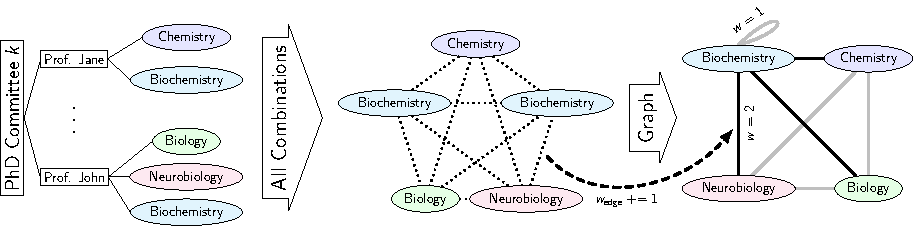
\includegraphics[width=\textwidth]{../poster/tikzout/vis_challenge_2018_poster-matthew_epland-figure0.pdf}
  \caption{Schematic representation of the method used to build the weighted academic organizations graph. Two members from a single committee are illustrated for example, but the method is applied to all committees and all members in practice.}
  \label{fig:method_schematic}
\end{figure}


\subsection{Finding Communities}
The academic organizations graph naturally contains sub-groups, or communities, of related disciplines, such as the Physical Sciences or Liberal Arts. These communities can be constructed algorithmically via the Louvain method \cite{louvain} which optimizes the graph's modularity, a measure of the density of interior to exterior edges of the component communities. The modularity $Q$ of graph $G$ can be defined as in (\ref{eq:modularity}) where $w_{ij}$ is the edge weight between organization nodes $i$ and $j$, $W_{i}$ is the sum of edge weights of node $i$, $W_{\mathrm{G}}$ is the total edge weight of the graph, and $c_{i}$ is the community of node $i$.

\begin{equation} \label{eq:modularity}
Q\left(G\right) = \frac{1}{2 W_{\mathrm{G}}} \sum_{ij \in G} \bigg(w_{ij} - \frac{W_{i} W_{j}}{2 W_{\mathrm{G}}}\bigg) \delta\left(c_{i},\,c_{j}\right)
\end{equation}

In this work the Louvain method was implemented via the \texttt{python-louvain} package \cite{python-louvain} with the resolution parameter\footnote{A resolution of $1$ corresponds to the standard Louvain method, while diverging from $1$ favors communities of different sizes. Other values were tested, but the best results were obtained with a resolution of $1$.} set at the default value of $1$.


\subsection{Measuring Interdisciplinary Activity}
To measure the interdisciplinary activity of each academic organization a straightforward interdisciplinary fraction $f$ of external and self connections was utilized (\ref{eq:intdisfrac}). Here $w_{\text{external}}$ is the sum of external edge weights of an organization's node, while $w_{\text{self}}$ is the weight of the edge from the node to itself. Binning the academic organizations graph by academic year\footnote{With bin edges: 2012--5--1, 2013--8--26, 2014--8--25, 2015--8--24, 2016--8--29, 2017--10--1} it is possible to see how $f$ changes for an organization over time.

\begin{equation} \label{eq:intdisfrac}
f = w_{\text{external}} / \big(w_{\text{external}} + w_{\text{self}}\big)
\end{equation}

$f$ works well for Ph.D.\ granting organizations with good statistics, but frequently breaks down with a value of $f=1.0$ for non-Ph.D.\ granting organizations as they do not have multiple faculty members sitting together on their own Ph.D.\ committees. To help remove such cases from consideration it is required that $w_{\text{total}} = w_{\text{external}} + w_{\text{self}} > 100$ per year, and that an organization have $\geq 3$ such years before being displayed.


%%%%%%%%%%%%%%%%%%%%%%%%%%%%%%%%%%%%%%%%%%%%%%%%%%%%%%%%%%%%%%%%%%%%%%%%%%%%%%%%%%%%%%%%%%%%%%%%%%%%
\section{Results}
\subsection{Academic Organizations Graph}

In addition to being the base object for later analysis, the academic organizations graph for all years, Figure~\ref{fig:graph_all_years}, provides a useful high-level view of the interdisciplinary networks at Duke. At a glance one can see how tightly linked organizations form the core of communities with smaller organizations on the periphery, and the relative separation between the science and medical communities and the liberal arts. The respective graphs for each academic year may be found in Appendix~\ref{appendix:graphs_by_year}.

\begin{figure}[!htb]\centering
  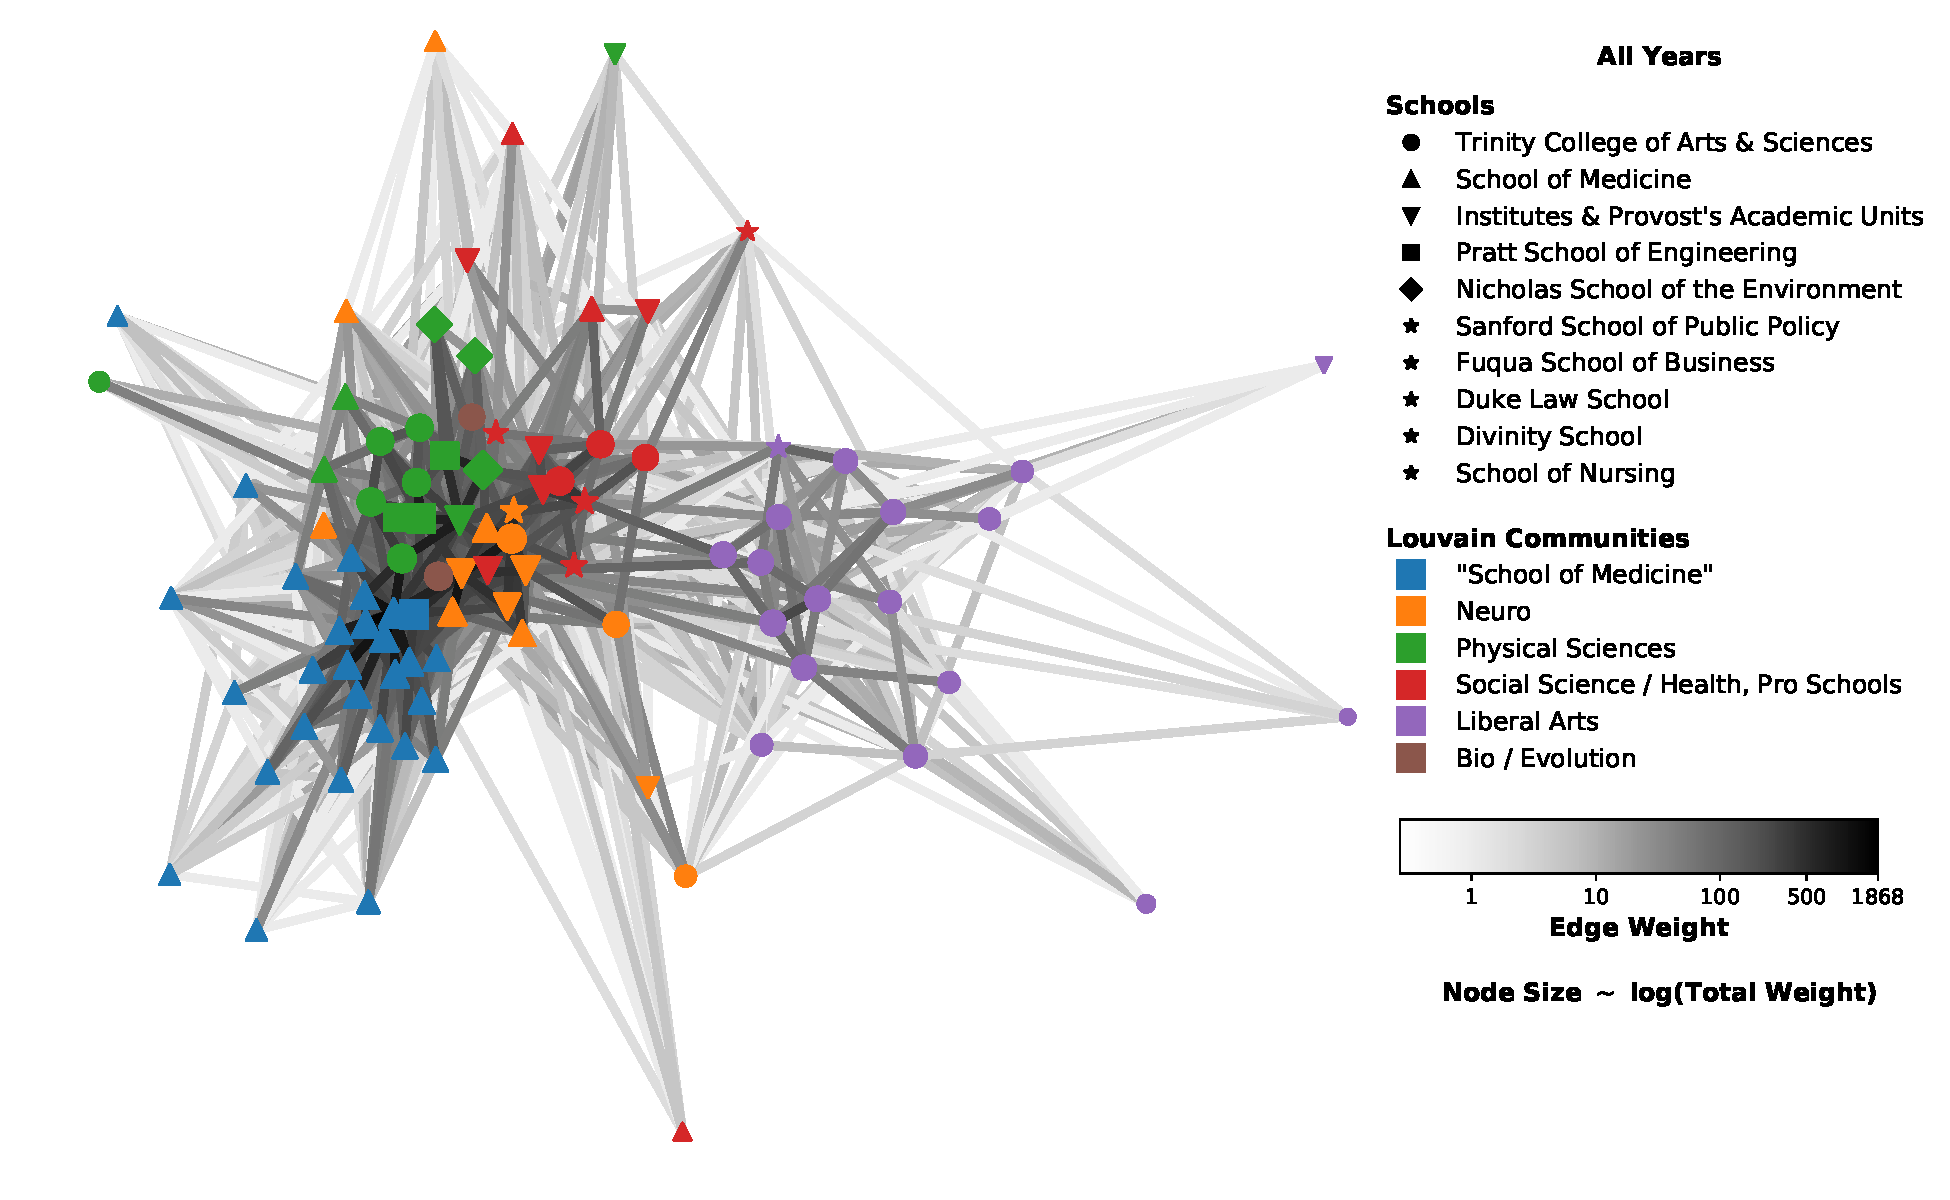
\includegraphics[width=\textwidth]{\figures/network_all_annotated.pdf}
  \caption{Academic organizations graph for all years.}
  \label{fig:graph_all_years}
\end{figure}

The graph for all years may also be viewed interactively online\footnote{\url{http://bl.ocks.org/mepland/raw/ee7d644c613d1ba18289f72d3f1b3456/}}, displayed with the \texttt{visJS2jupyter} package \cite{visJS2jupyter}. There additional details on each node and edge may be viewed by hovering over them, and the nodes may be dragged into new positions to better examine certain areas.
% TODO make sure url is correct in the end!


\subsection{Communities}
When run on the academic organizations graph for all years, the Louvain method found 6 communities of varying sizes. Each community was then named based on its constituent organizations; ``School of Medicine'', Neuro, Physical Sciences, ``Social Science / Health, Pro Schools'', Liberal Arts, Bio / Evolution. Most communities contained the organizations one would expect from their given names, with a few random additions. The large Neuro cluster pulling organizations from multiple schools across campus was an interesting find, along with the insular Biology / Evolutionary Anthropology paring that surprisingly did not connect with any other community despite several appearing compatible from a traditional disciplinary point of view. See Appendix~\ref{appendix:community_members} for a complete listing of organizations in each community.


\subsection{Interdisciplinary Activity}
The interdisciplinary fraction $f$ vs year was plotted for the top 10 organizations by total weight in each community, see Figures~\ref{fig:interdis_frac_physical_sciences}--\ref{fig:interdis_frac_liberal_arts} for three interesting examples.

\begin{figure}[!htb]\centering
  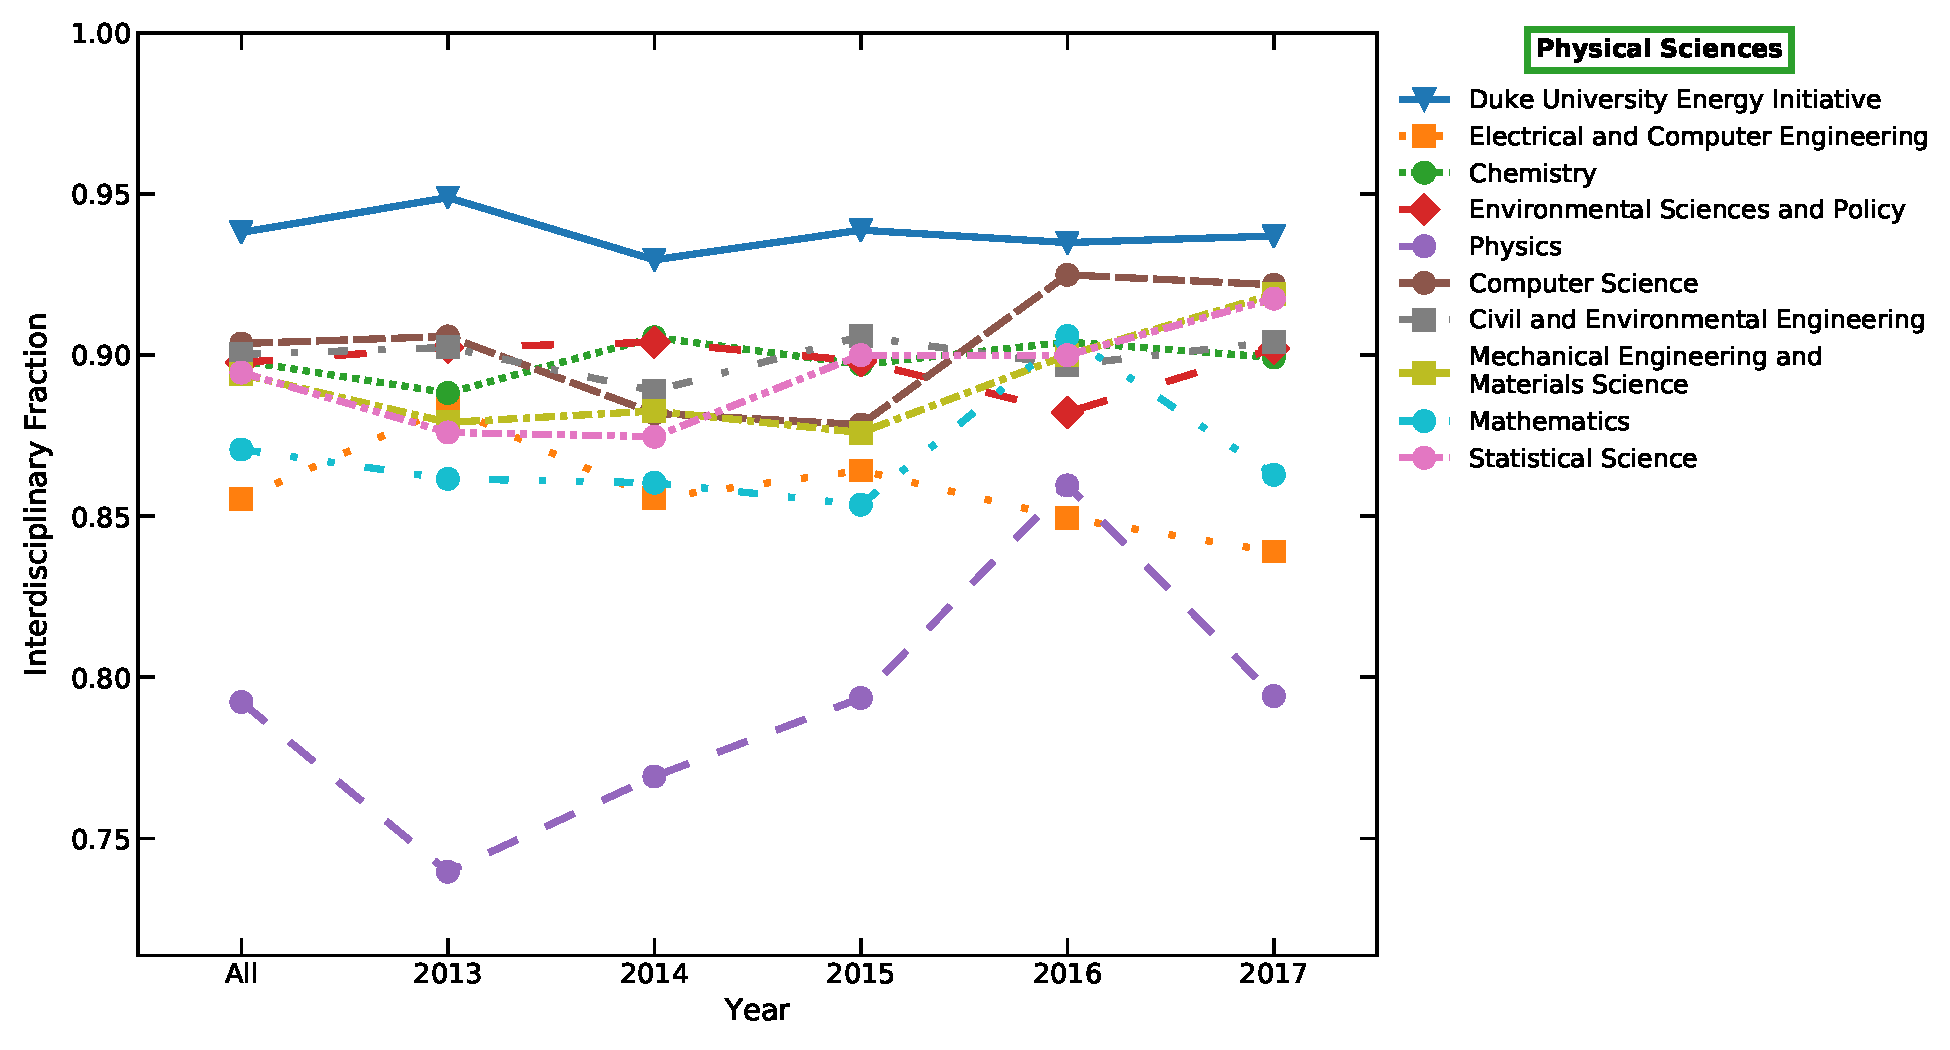
\includegraphics[width=\textwidth]{\figures/interdis_frac/communities/Physical_Sciences.pdf}
  \caption{Interdisciplinary fraction vs year for the Physical Sciences community.}
  \label{fig:interdis_frac_physical_sciences}
\end{figure}

\begin{figure}[!htb]\centering
  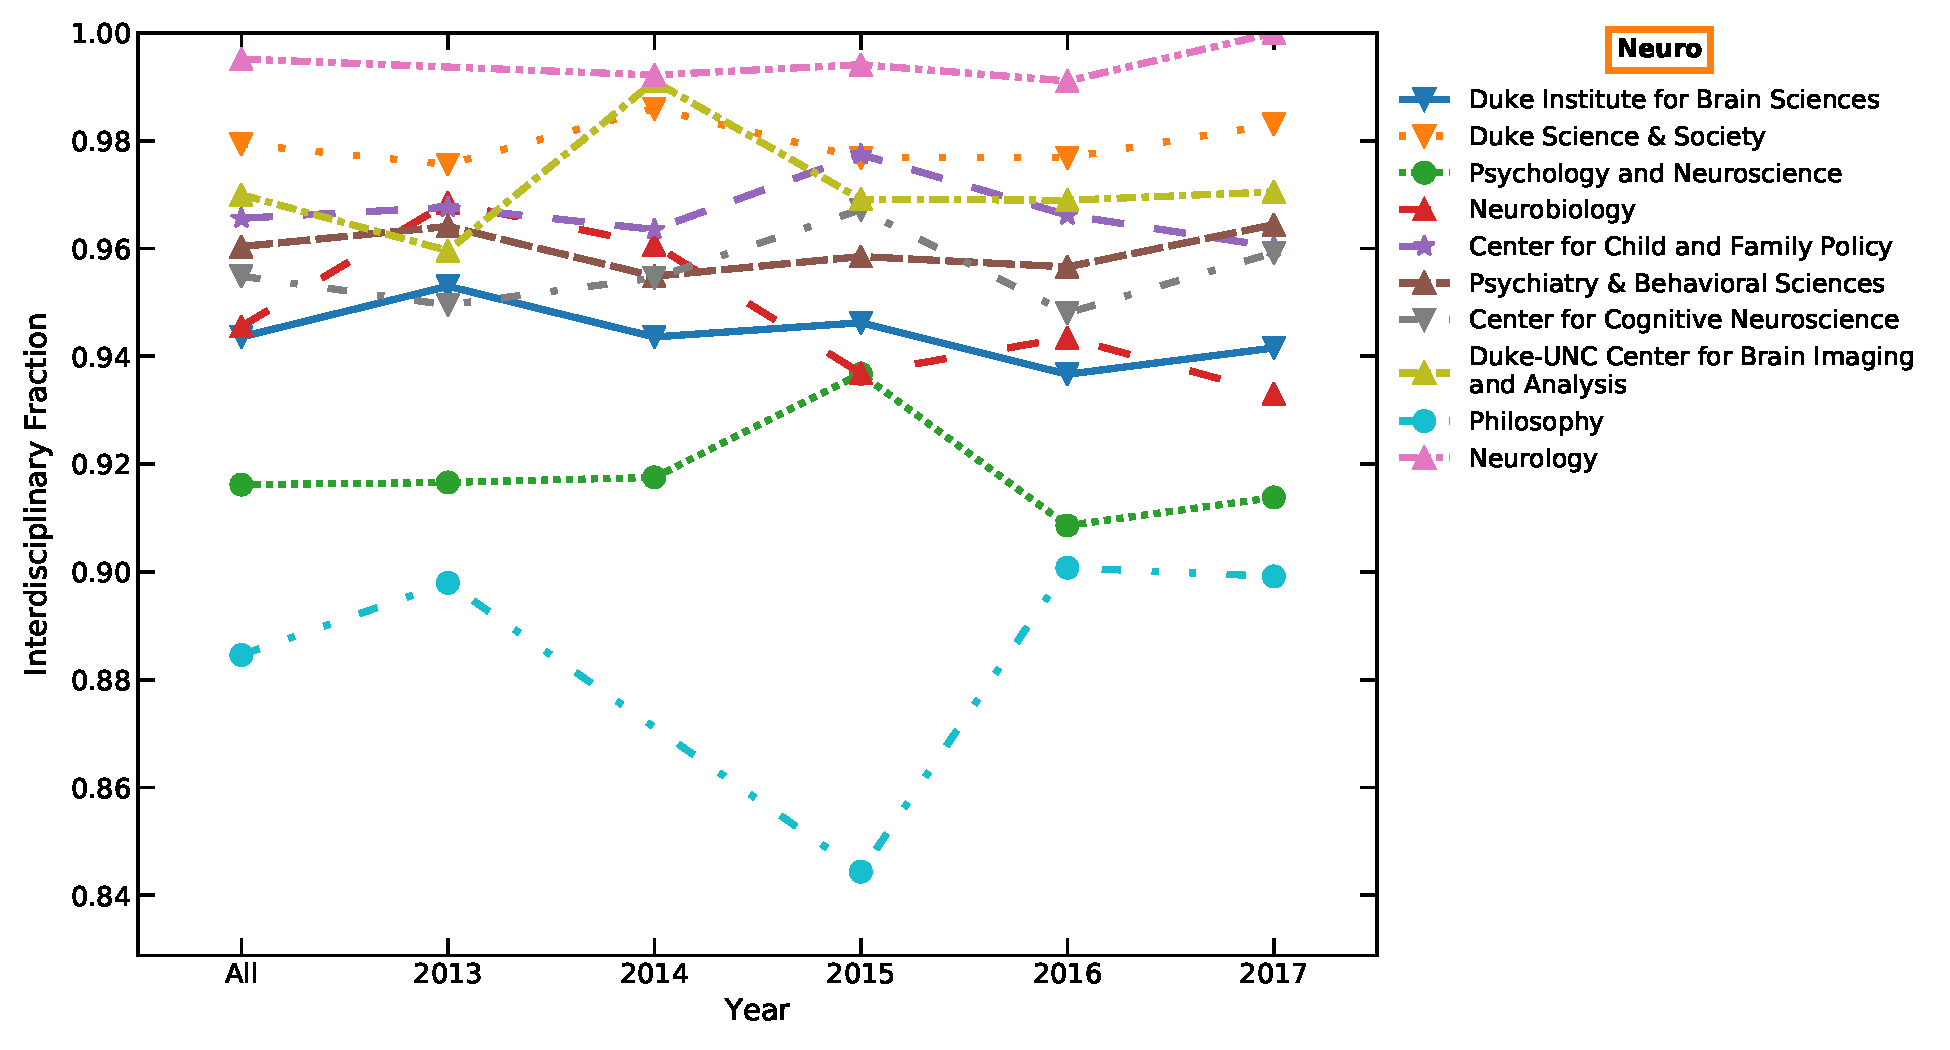
\includegraphics[width=\textwidth]{\figures/interdis_frac/communities/Neuro.pdf}
  \caption{Interdisciplinary fraction vs year for the Neuro community.}
  \label{fig:interdis_frac_neuro}
\end{figure}

In the Physical Sciences community the majority of the top 10 organizations had fairly steady $f \approx 90-95\%$, with the exception of Physics which had wide variations between $f \approx 75-90\%$. In the Neuro community the majority of organizations fell a bit higher at $f \approx 94-98\%$, with Psychology and Neuroscience, and Philosophy varying between $f \approx 84-94\%$. The lower $f$ values and increased year-to-year variations in the Physics, Psychology and Neuroscience, and Philosophy departments is intriguing and warrants further investigation. Two hypotheses for why they behave differently from their peers is that these departments have stricter policies regarding faculty joint and secondary appointments in other departments, or including multiple Ph.D.\ committee members from outside the field. Further analysis efforts described in Section~\ref{sec:future} could help test these hypotheses, as would qualitatively evaluating the department cultures and policies.

\begin{figure}[!htb]\centering
  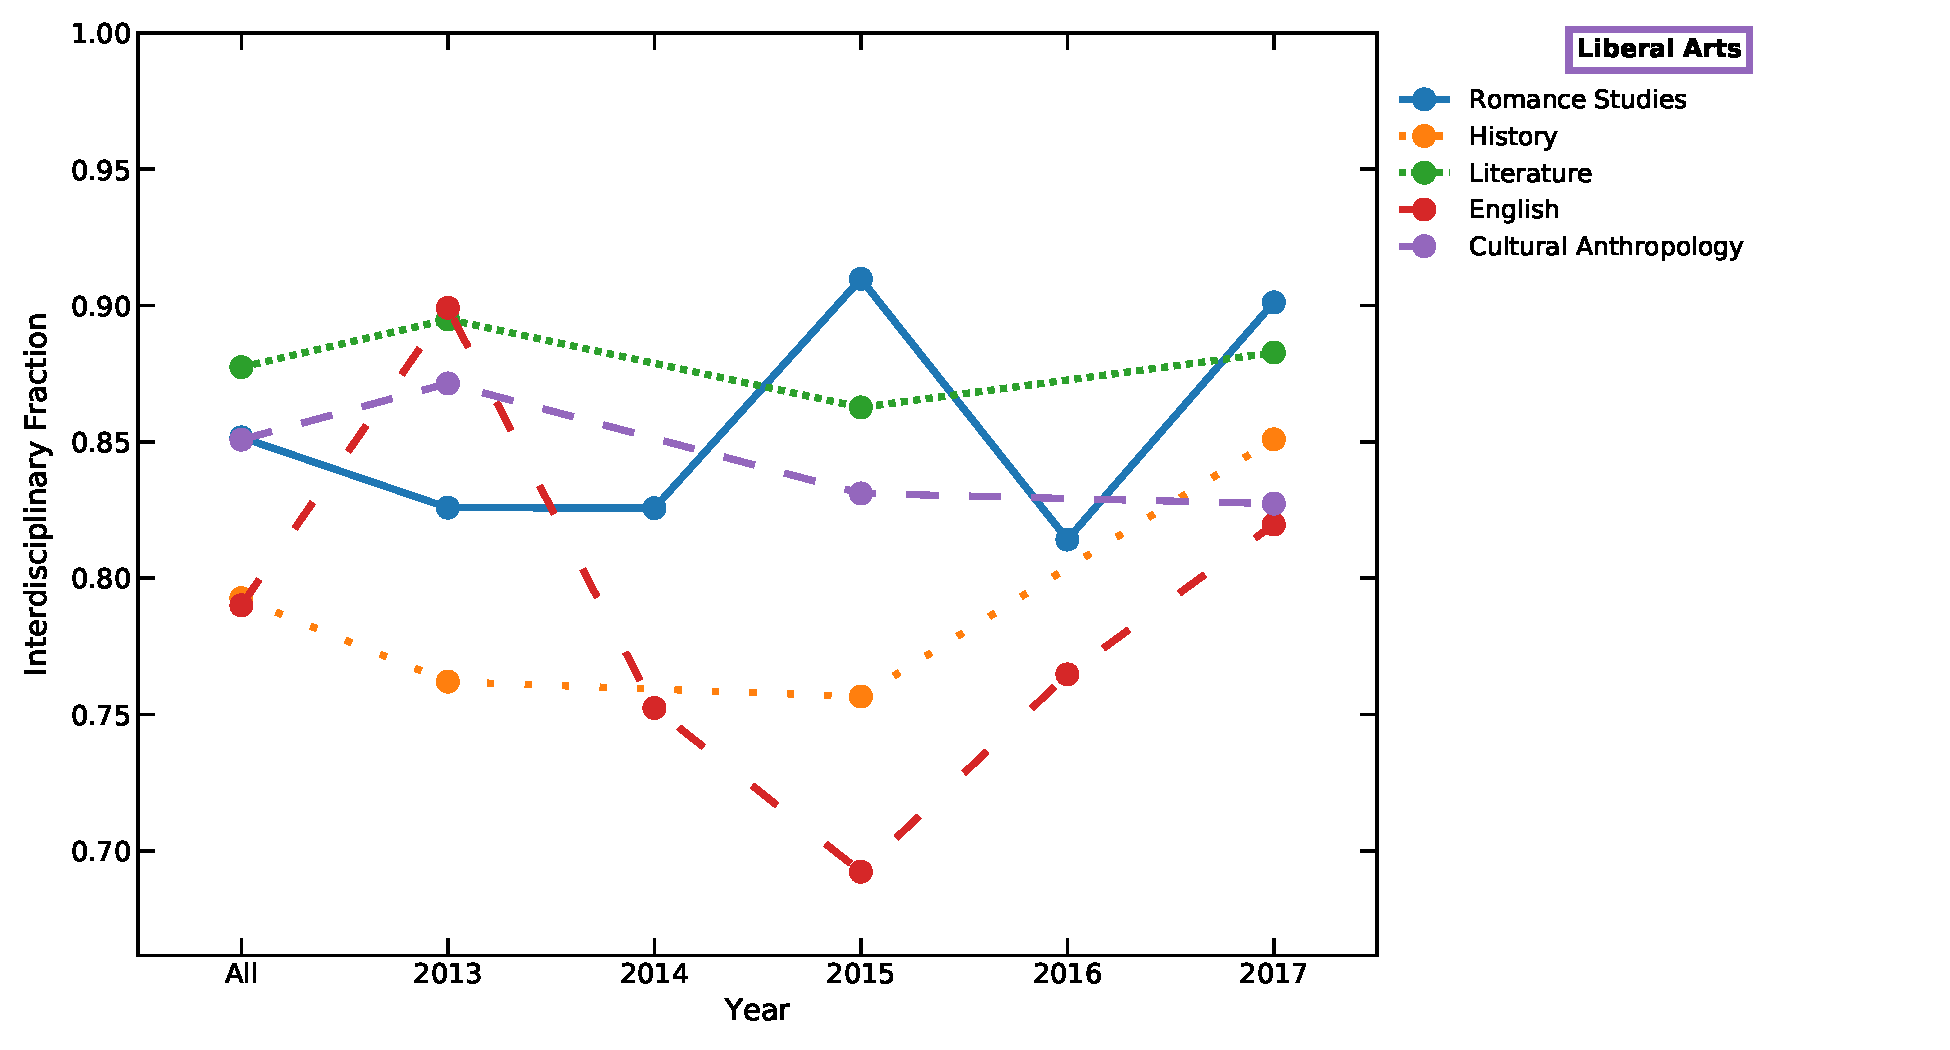
\includegraphics[width=\textwidth]{\figures/interdis_frac/communities/Liberal_Arts.pdf}
  \caption{Interdisciplinary fraction vs year for the Liberal Arts community.}
  \label{fig:interdis_frac_liberal_arts}
\end{figure}

In contrast to the Physical Sciences and Nero communities, organizations in the Liberal Arts were lower at $f \approx 75-90\%$, but suffered from low statistics which increased the variance and limited the number of organizations passing the weight cut to only 5. Additional data is needed from these organizations before usable comparisons between the sciences and Liberal Arts can be made.

The remaining plots of $f$ for each community can be found in Appendix~\ref{appendix:interdis_frac_community}. Additionally similar plots were produced for each school, see Appendix~\ref{appendix:interdis_frac_school}.


%%%%%%%%%%%%%%%%%%%%%%%%%%%%%%%%%%%%%%%%%%%%%%%%%%%%%%%%%%%%%%%%%%%%%%%%%%%%%%%%%%%%%%%%%%%%%%%%%%%%
\section{Potential Issues and Future Improvements}
\label{sec:future}
Due to time constraints imposed by the challenge a number of potential issues and improvements to the analysis were identified but could not be investigated. They are listed here for completeness and for possible use in the future. Note that some solutions presented here should improve multiple aspects of the analysis simultaneously.

\subsubsection{Non-Ph.D.\ Granting Academic Organizations Underrepresented}
As the \path{dissertation_committees_2012-2017.xlsx} dataset only contains information on Ph.D.\ committees, academic organizations such as professional schools who typically grant other kinds of graduate degrees, and interdisciplinary institutes and centers who do not directly grant graduate degrees of any kind, are underrepresented. This leads to poor statistics and frequent unrealistic $f=1.0$ break downs for these organizations.

An easy solution, provided the data is available, is to request and integrate the non-Ph.D.\ committee records from the graduate and professional schools. However this does not address the issues with organizations that do not grant any graduate degrees. A potentially wider solution is to switch datasets entirely and utilize the \path{ScholarsAtDuke_Publications_2012-2017.xlsx} publication data. There joint authorship on a paper could be used in the exact same way as joint membership on a committee to construct a new graph using much of the existing procedure and code, but would constitute essentially re-running the entire analysis.

\subsubsection{Effects of Joint and Secondary Appointments vs Committee Membership}
The academic organizations graph is currently constructed such that the weight added to an edge of two organizations connected from one faculty member holding appointments in each ($w=1$) is the same as the weight added to an edge from two faculty members with different appointments serving on the same Ph.D.\ committee. While there is nothing incorrect with this method a priori, there also is no outside reason for it. Alternative weighting schemes should be devised and tested to determine what works best for this dataset and analysis. Another round of elicitation from the relevant stakeholders would be helpful when forming metrics on which to test the weighting schemes\footnote{For example, if a department has restrictive policies regarding joint and secondary appointments, should that be taken as a sign of non-interdisciplinary activity, or be guarded against as a possible source of bias?}, as holding multiple appointments and sitting on an interdisciplinary committee are both indicators of interdisciplinary activity.

Two weighting schemes were in fact tested during development, one which only considered primary appointments and the second as presented here in Section~\ref{sec:construct_graph} which weighted primary, joint and secondary appointments equally. The second method was ultimately chosen as it produced a more interconnected graph with reasonable Louvain communities. Other possible weighting schemes to test include weighting joint and secondary appointments at a constant value less than primary appointments, and normalizing the weights per faculty member such that their primary appointment receives a weight of $0.5$\footnote{Or $1$ if they only hold a primary appointment and $n=0$.} while any $n$ joint and secondary appointments receive $0.5 / n$ such that each faculty member only contributes a maximum combined weight of $1$.

\subsubsection{Improved Data Cleaning}
As implemented the process to clean and merge the committee and faculty datasets is fairly strict. Everything is done by the DUID number and if there is a missing or mismatched record the faculty member, or even committee, will be dropped. Some of these cases may be caused by recently retired faculty appearing on past committees, but not in \path{ScholarsAtDuke_Faculty_October2017.xlsx}; the solution here is to acquire a larger dataset of all faculty from 2012--2017. Others may be due to non-Duke faculty serving as committee members, which is probably intractable with the Duke only sources of data available\footnote{Baring some extensive web and publication scrapping effort.}. Lastly, some faculty mismatches may be the simple result of clerical errors when entering the DUID\footnote{A handful of committee members have DELETE in their names, so this is a real possibility.}, in this case a semi-autonomous fallback function could be developed to try to match faculty by name.

The additional effort needed to improve the data cleaning may not be worth the increased statistics in the end --- particularly if large amounts of new data is acquired yearly. However, it should at least be studied as a potential source of bias as some academic organizations may be systematically affected by one or more of the above DUID data quality issues.


%%%%%%%%%%%%%%%%%%%%%%%%%%%%%%%%%%%%%%%%%%%%%%%%%%%%%%%%%%%%%%%%%%%%%%%%%%%%%%%%%%%%%%%%%%%%%%%%%%%%
\section{Conclusions}
The nature of interdisciplinary research at Duke was explored at the departmental level by studying connections found in Ph.D.\ committees from the academic years of 2013--2017. Communities of related academic organizations where created via the Louvain method, most following the typical disciplinary distinctions with a few interesting exceptions in Neuro community and Biology / Evolutionary Anthropology paring. The interdisciplinary activity of individual organizations was investigated via the development of interdisciplinary fraction $f$, which revealed lower values of $f$ for the Physics, Psychology and Neuroscience, and Philosophy departments. Future directions and areas of improvement for the analysis where identified, along with possible solutions. 


%%%%%%%%%%%%%%%%%%%%%%%%%%%%%%%%%%%%%%%%%%%%%%%%%%%%%%%%%%%%%%%%%%%%%%%%%%%%%%%%%%%%%%%%%%%%%%%%%%%%
%%%%%%%%%%%%%%%%%%%%%%%%%%%%%%%%%%%%%%%%%%%%%%%%%%%%%%%%%%%%%%%%%%%%%%%%%%%%%%%%%%%%%%%%%%%%%%%%%%%%

\bibliographystyle{\includedir/bib/atlasBibStyleWithTitle}
\bibliography{\includedir/bib/bib.bib}

\newpage % TODo hard coded!
%%%%%%%%%%%%%%%%%%%%%%%%%%%%%%%%%%%%%%%%%%%%%%%%%%%%%%%%%%%%%%%%%%%%%%%%%%%%%%%%%%%%%%%%%%%%%%%%%%%%

\begin{appendices}


\section{Academic Organizations Graphs by Year}
\label{appendix:graphs_by_year}

\begin{figure}[!htb]\centering
  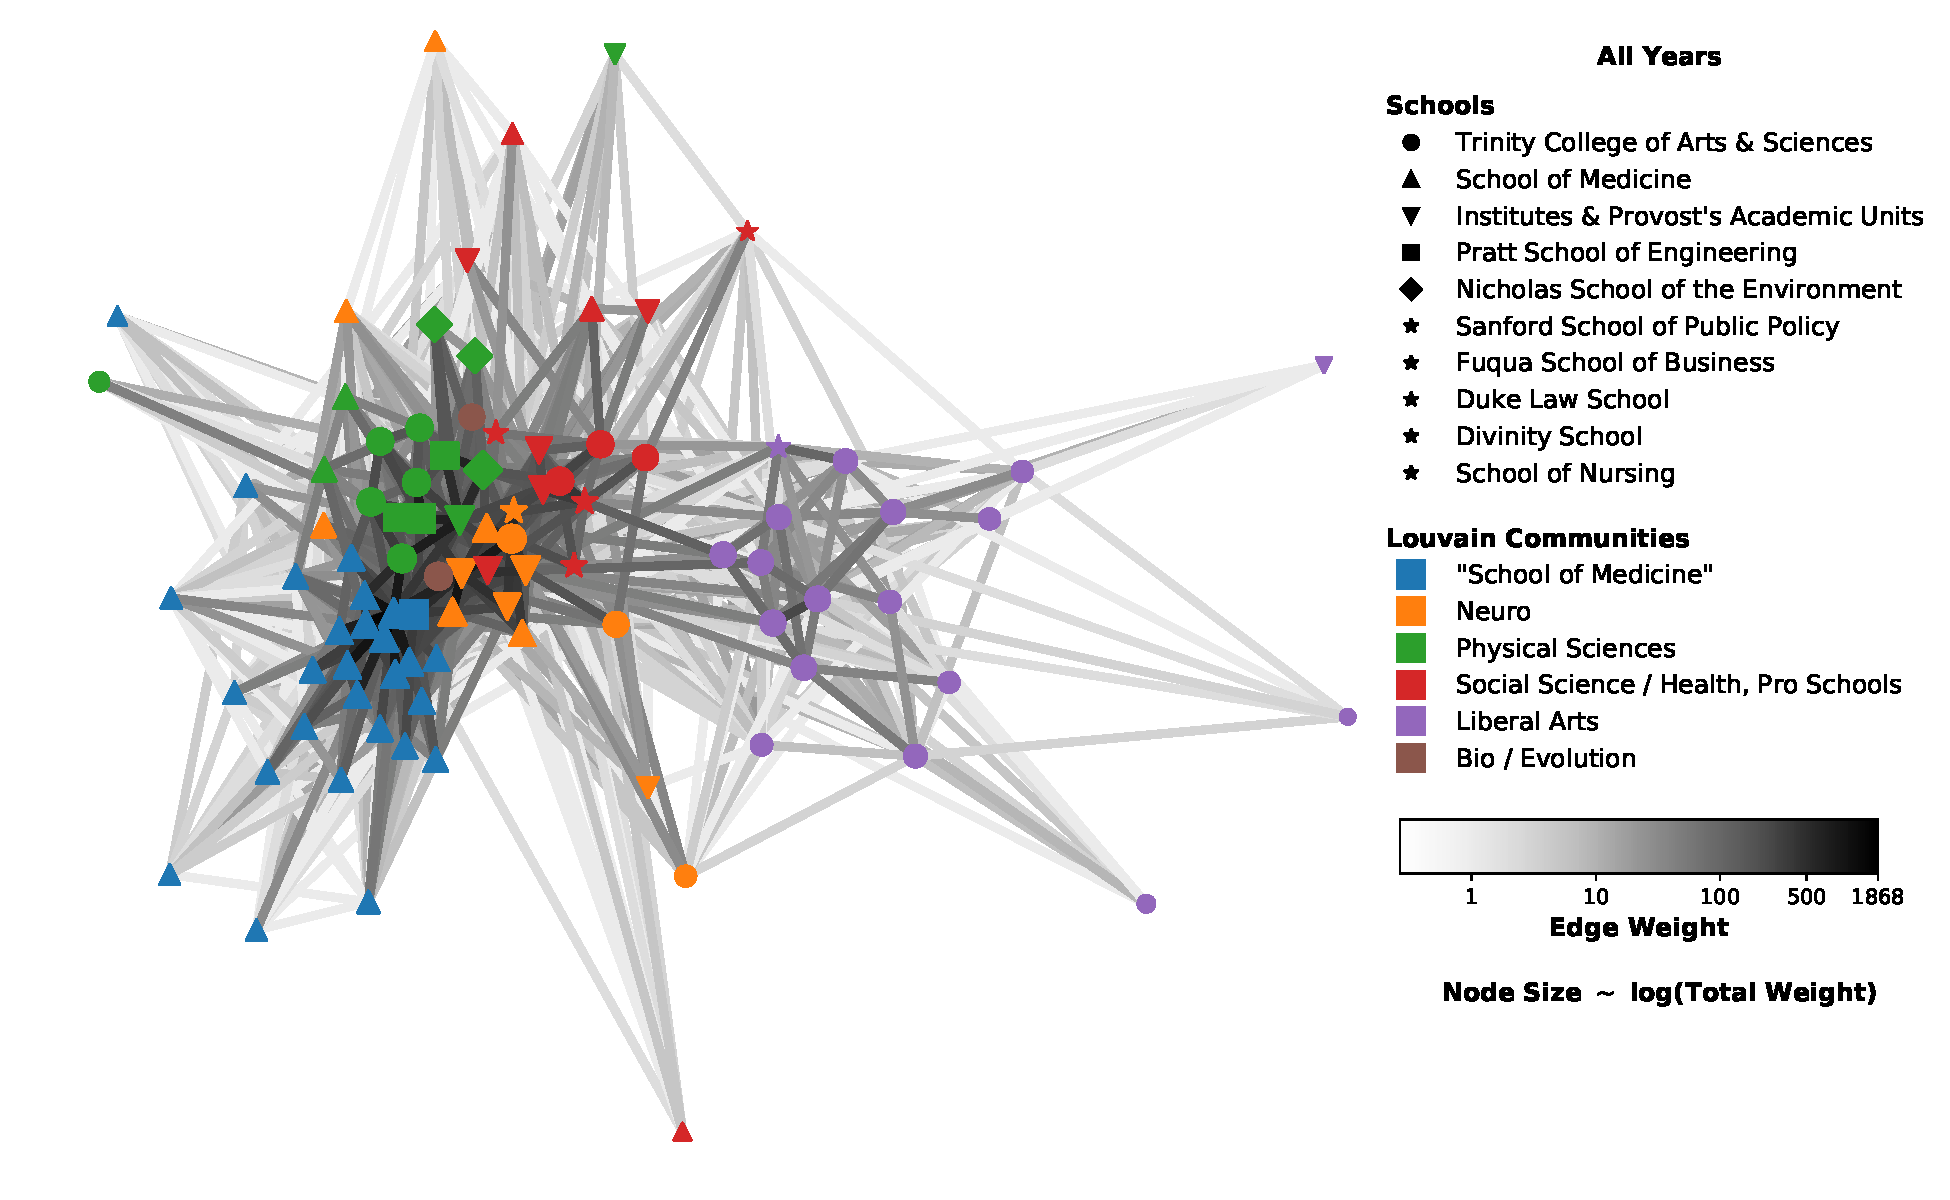
\includegraphics[width=\textwidth]{\figures/network_all_annotated.pdf}
  \caption{Academic organizations graph for all years. Figure~\ref{fig:graph_all_years} reproduced for convenience.}
\end{figure}

\vspace{-0.5cm}

\begin{figure}[!htb]\centering
  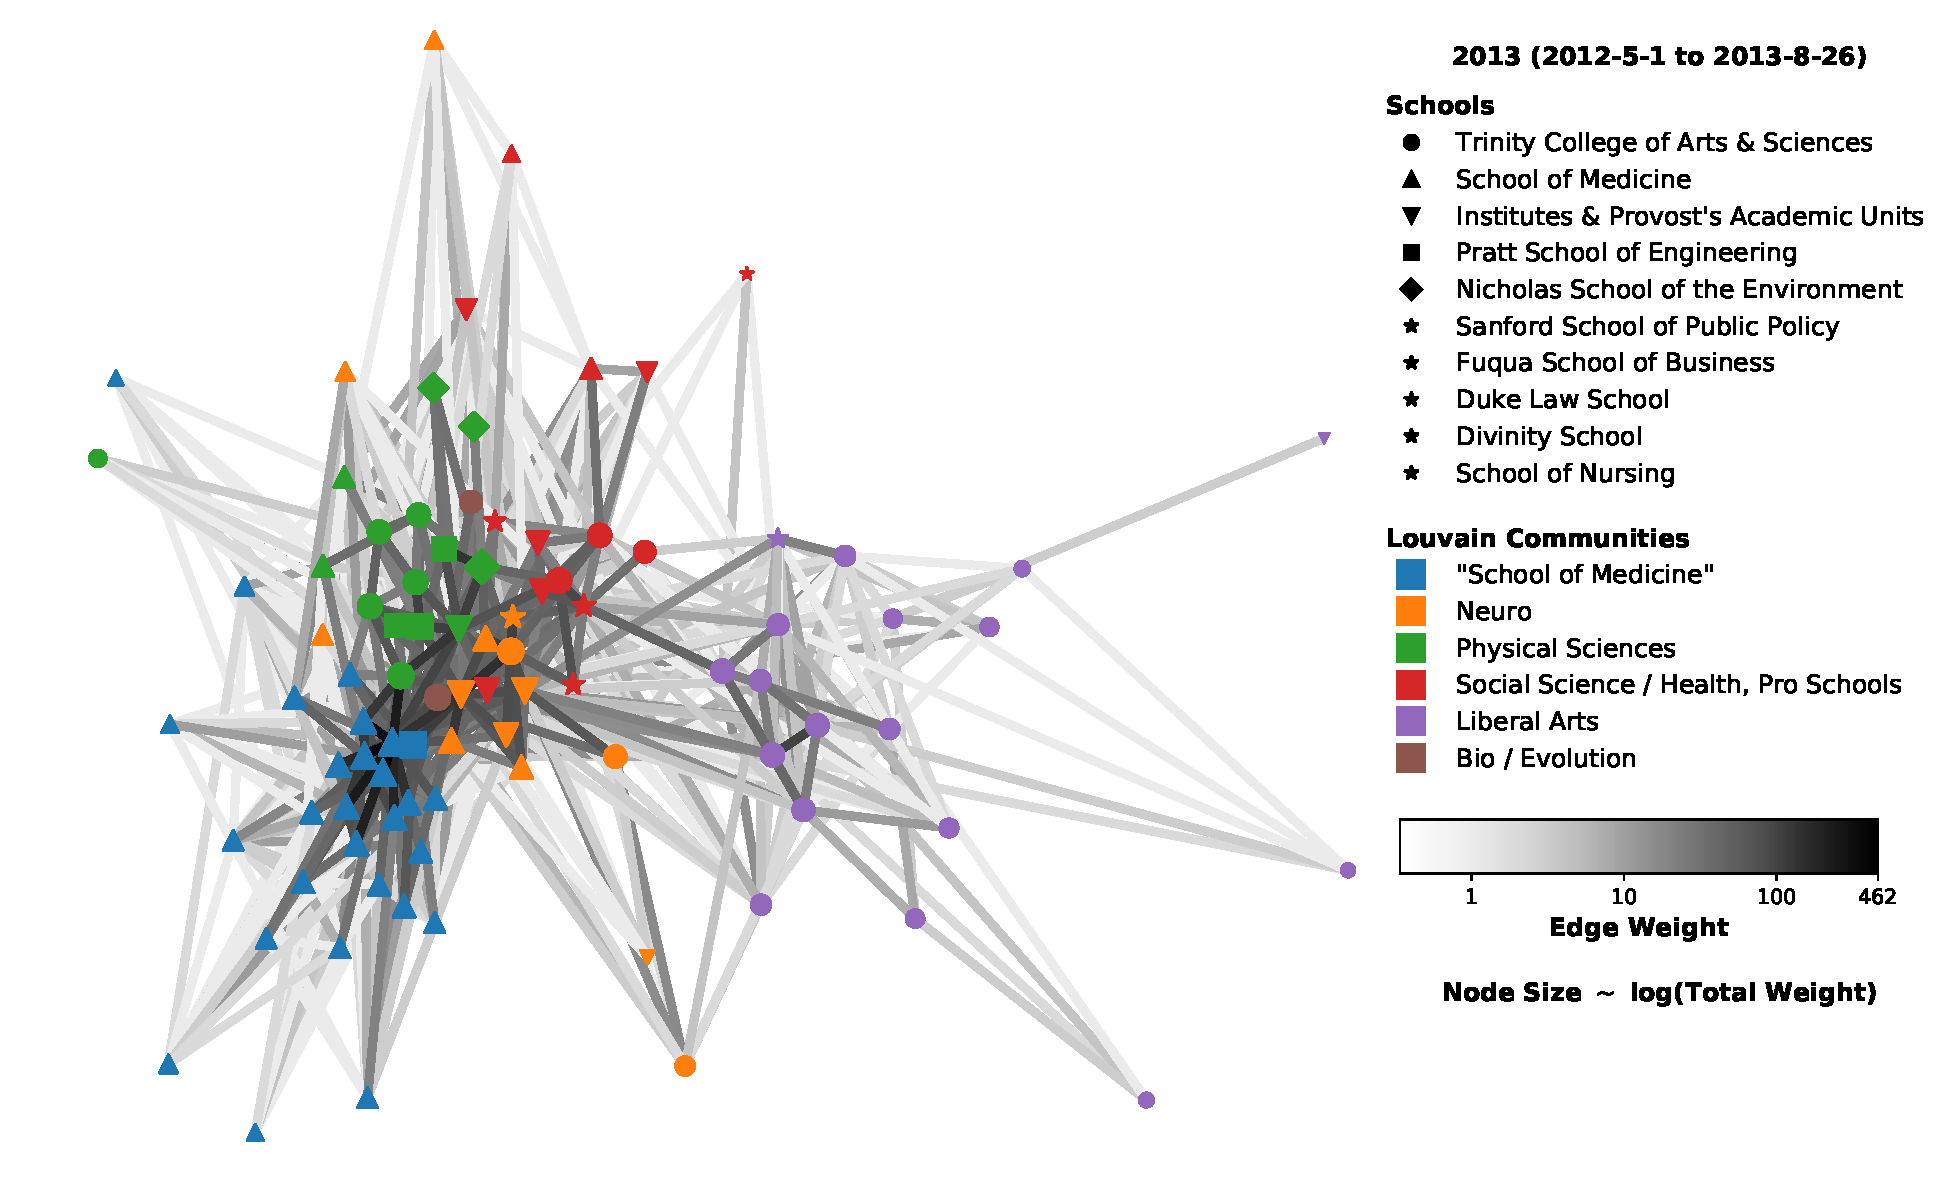
\includegraphics[width=\textwidth]{\figures/time_binned_networks/network_2013.pdf}
  \caption{Academic organizations graph for 2013.}
\end{figure}

\begin{figure}[!htb]\centering
  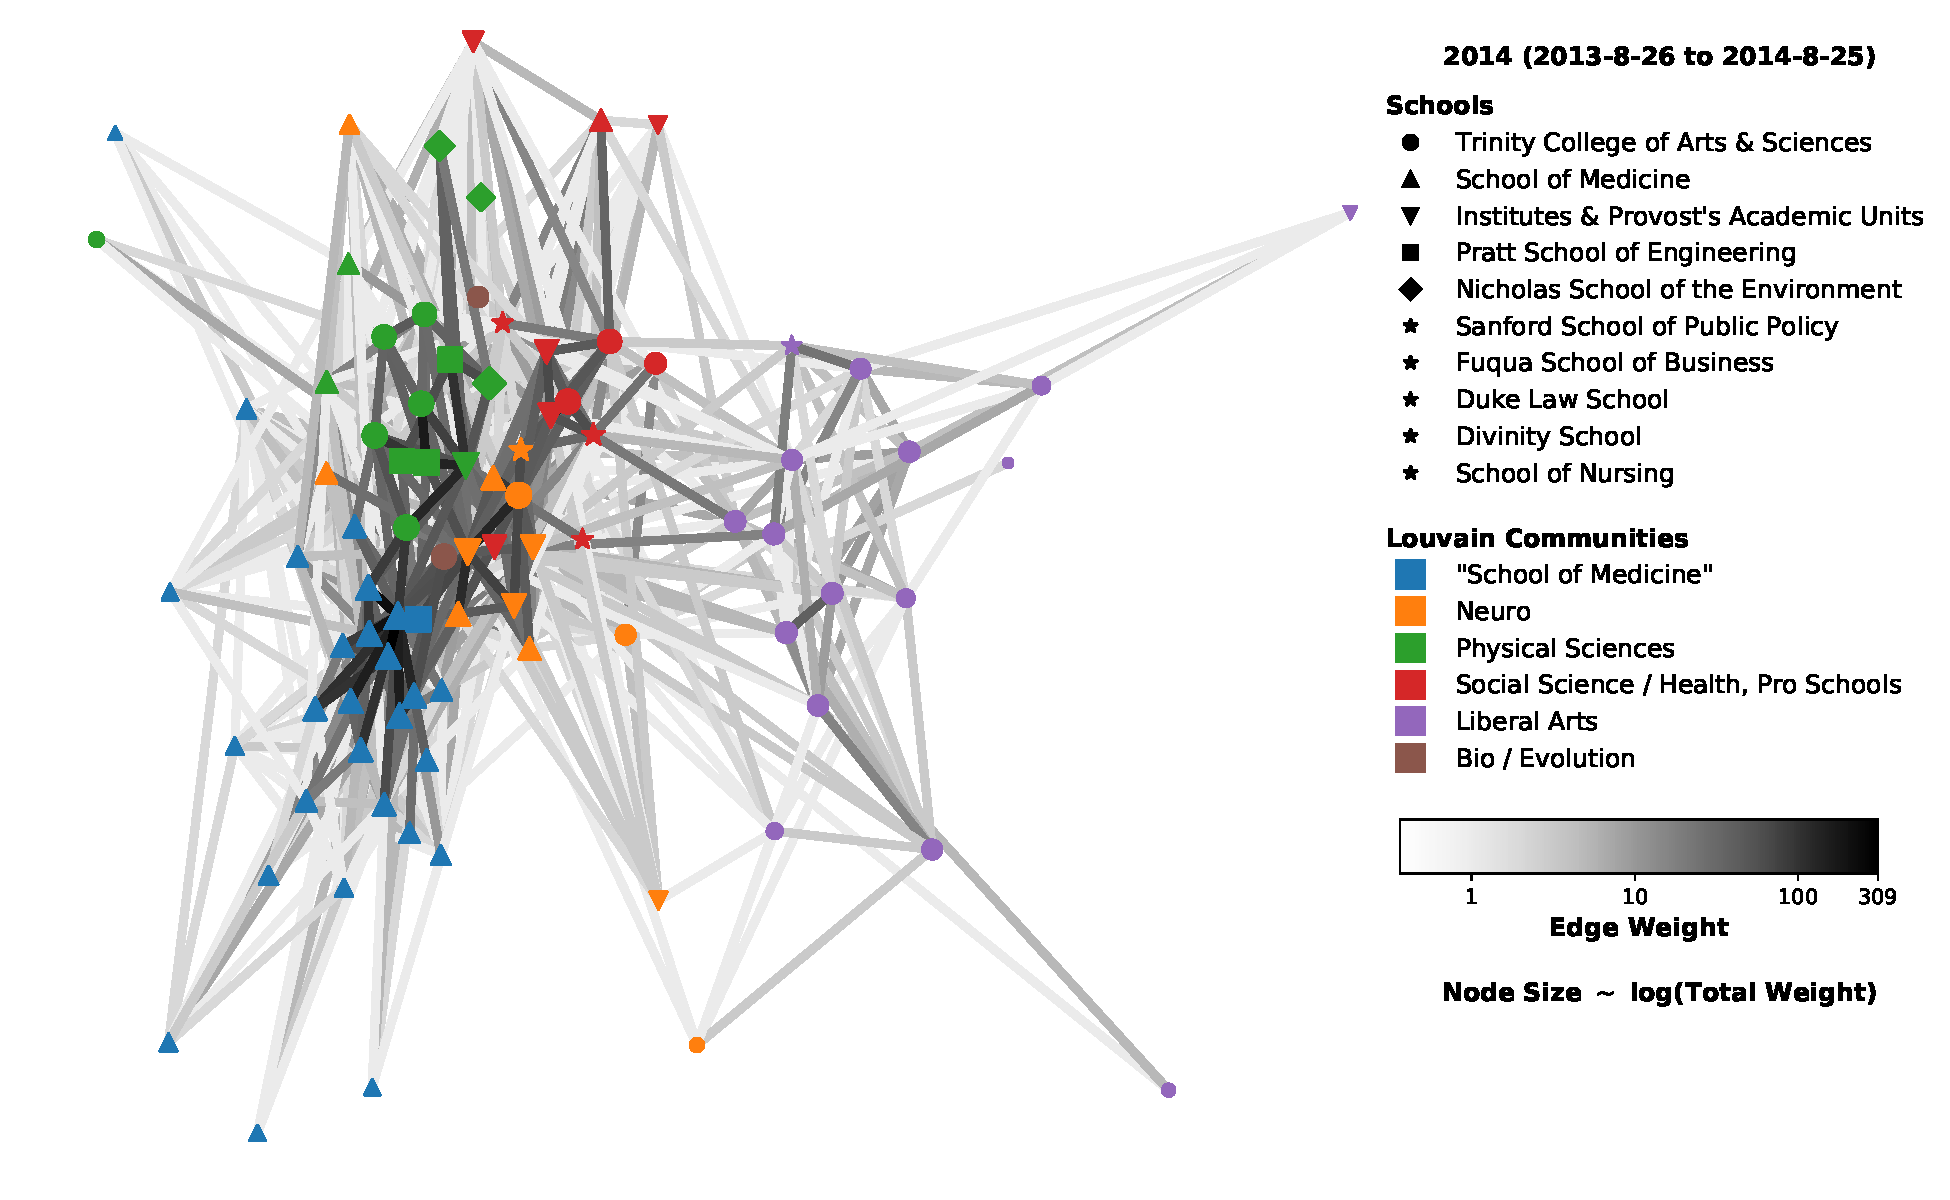
\includegraphics[width=\textwidth]{\figures/time_binned_networks/network_2014.pdf}
  \caption{Academic organizations graph for 2014.}
\end{figure}

\begin{figure}[!htb]\centering
  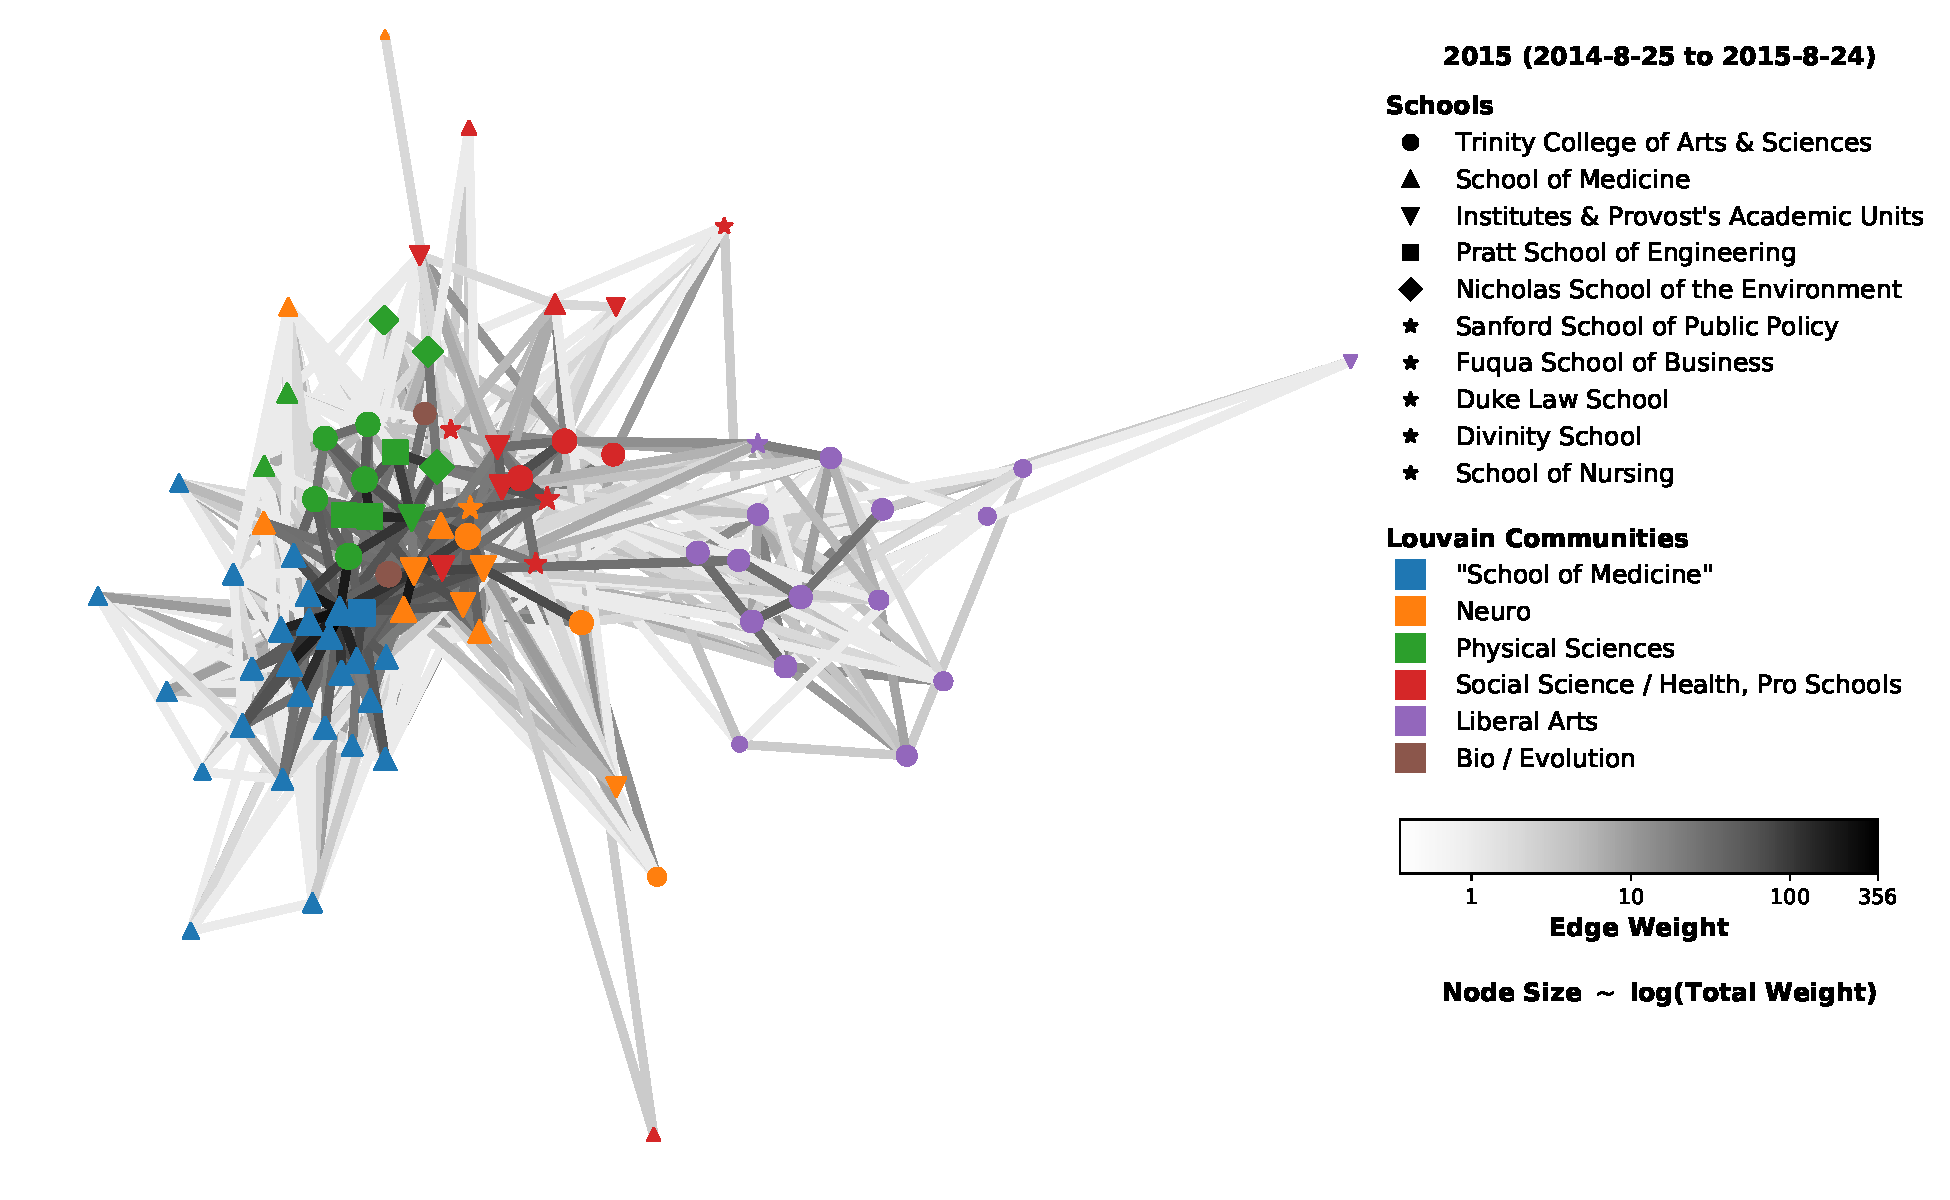
\includegraphics[width=\textwidth]{\figures/time_binned_networks/network_2015.pdf}
  \caption{Academic organizations graph for 2015.}
\end{figure}

\begin{figure}[!htb]\centering
  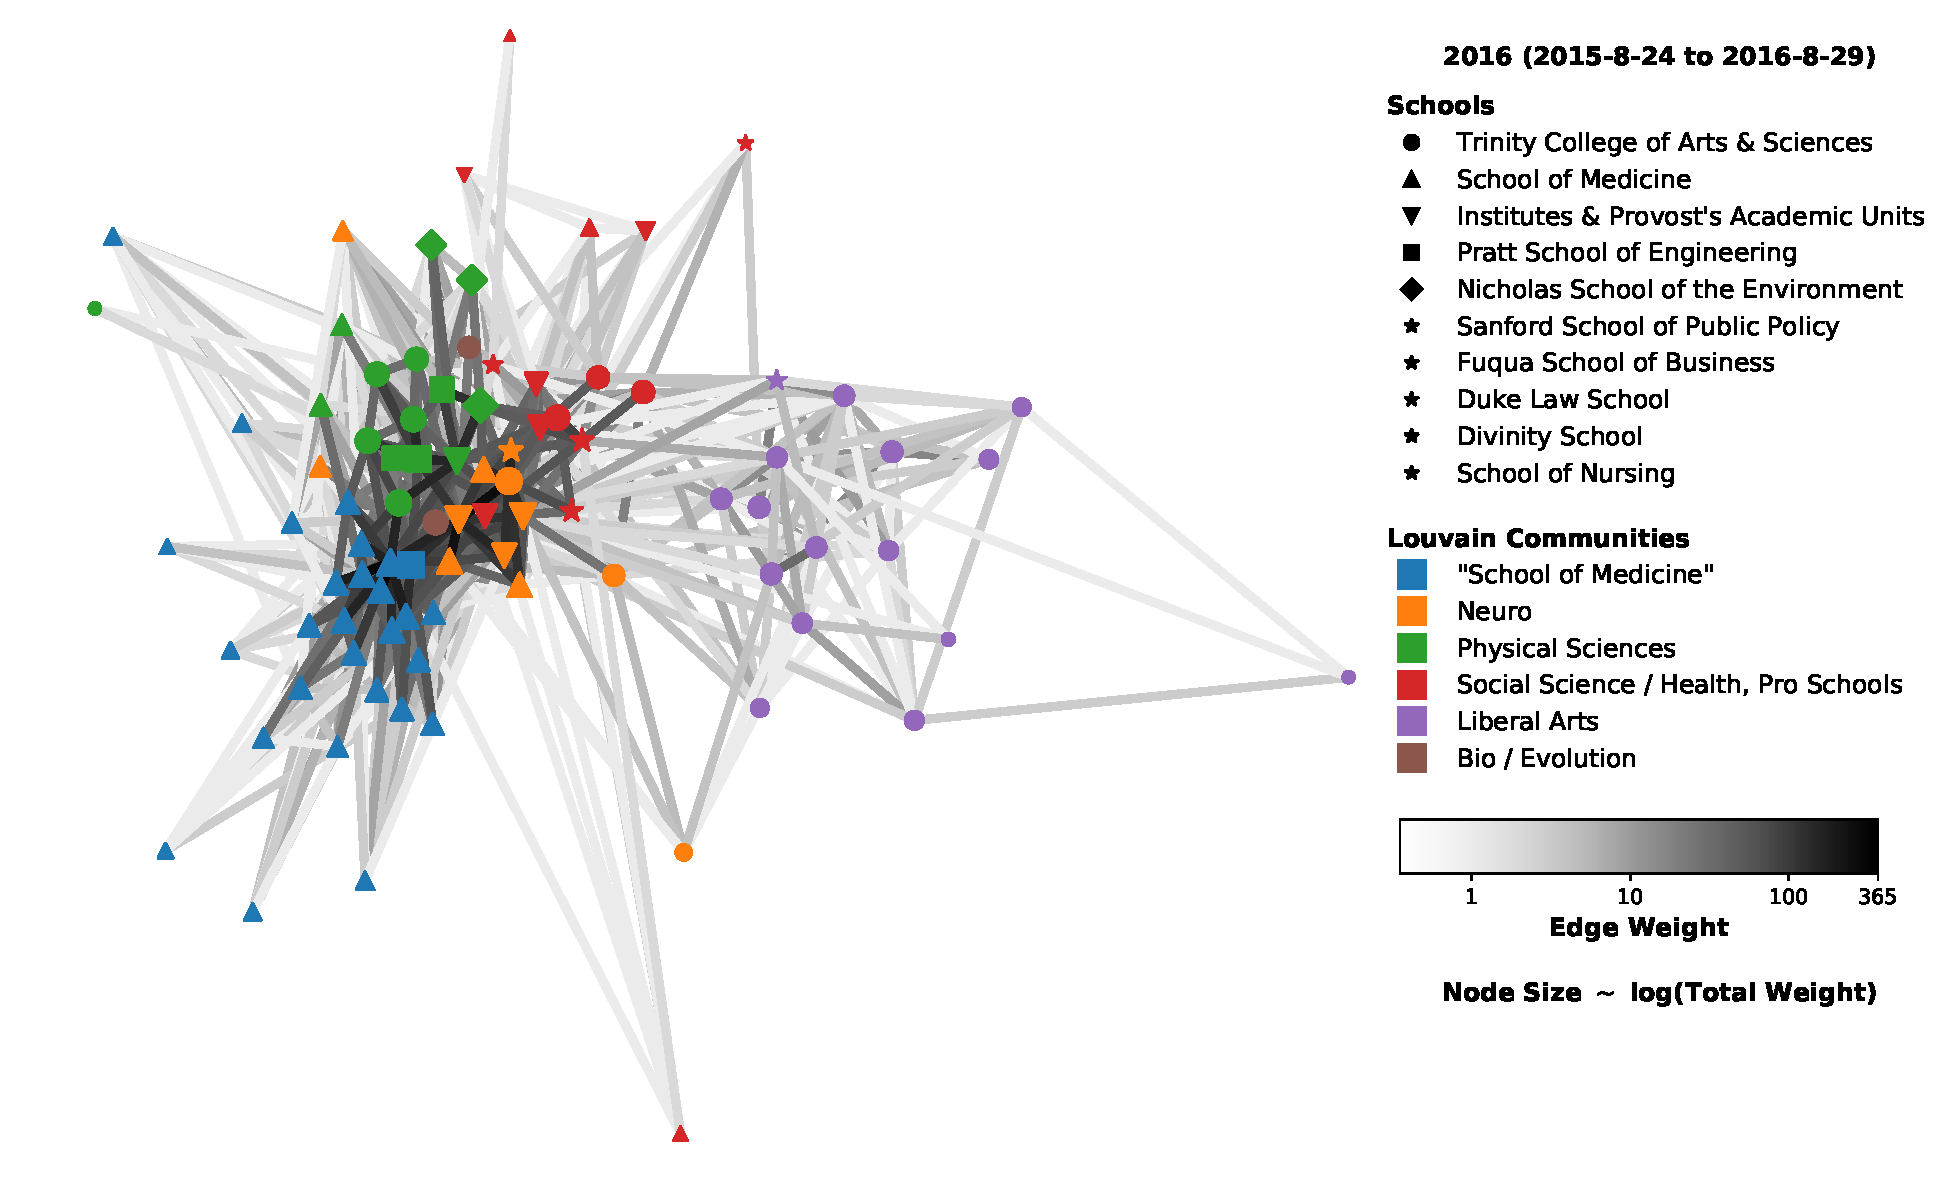
\includegraphics[width=\textwidth]{\figures/time_binned_networks/network_2016.pdf}
  \caption{Academic organizations graph for 2016.}
\end{figure}

\begin{figure}[!htb]\centering
  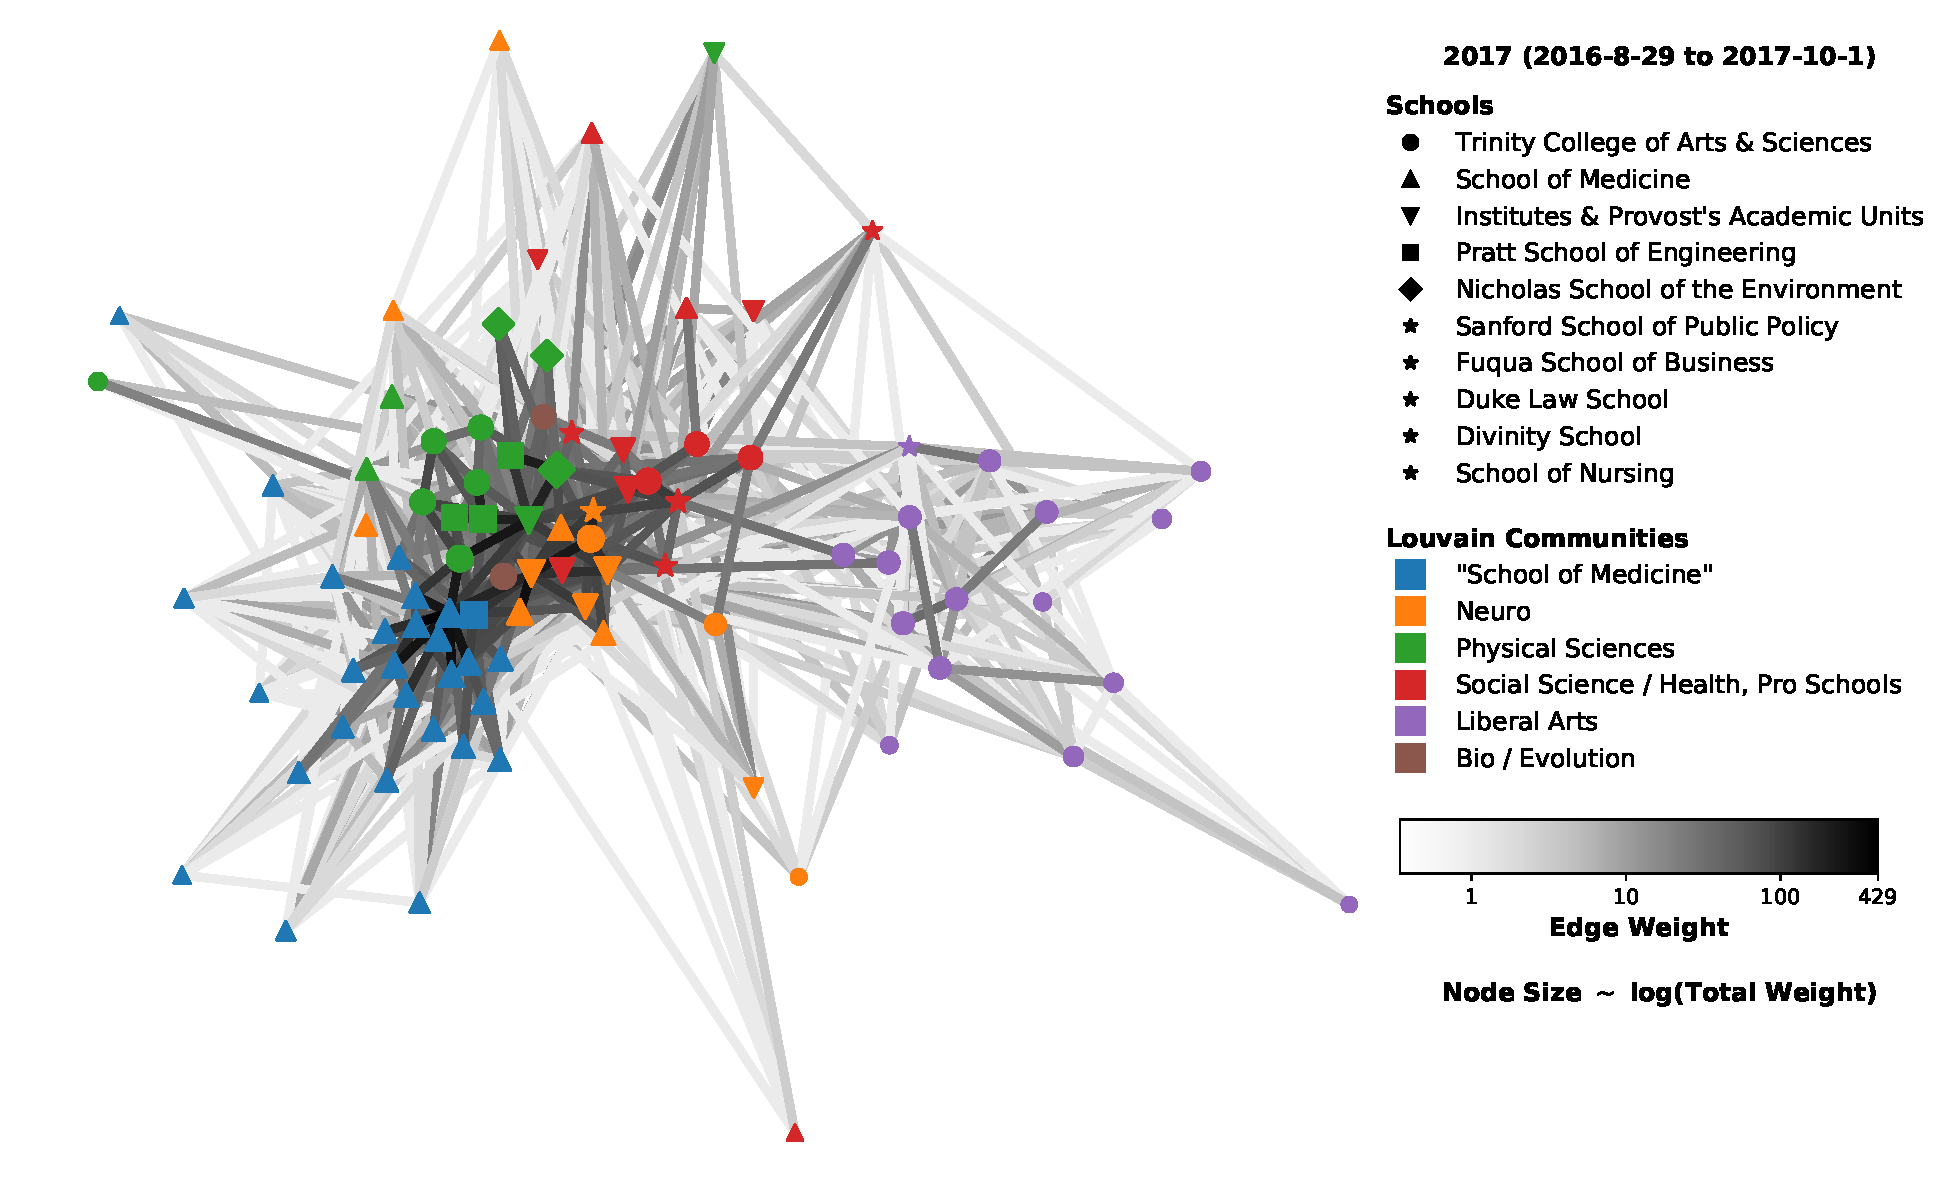
\includegraphics[width=\textwidth]{\figures/time_binned_networks/network_2017.pdf}
  \caption{Academic organizations graph for 2017.}
\end{figure}


\section{Louvain Community Members}
\label{appendix:community_members}

\begin{figure}[!htb]\centering
  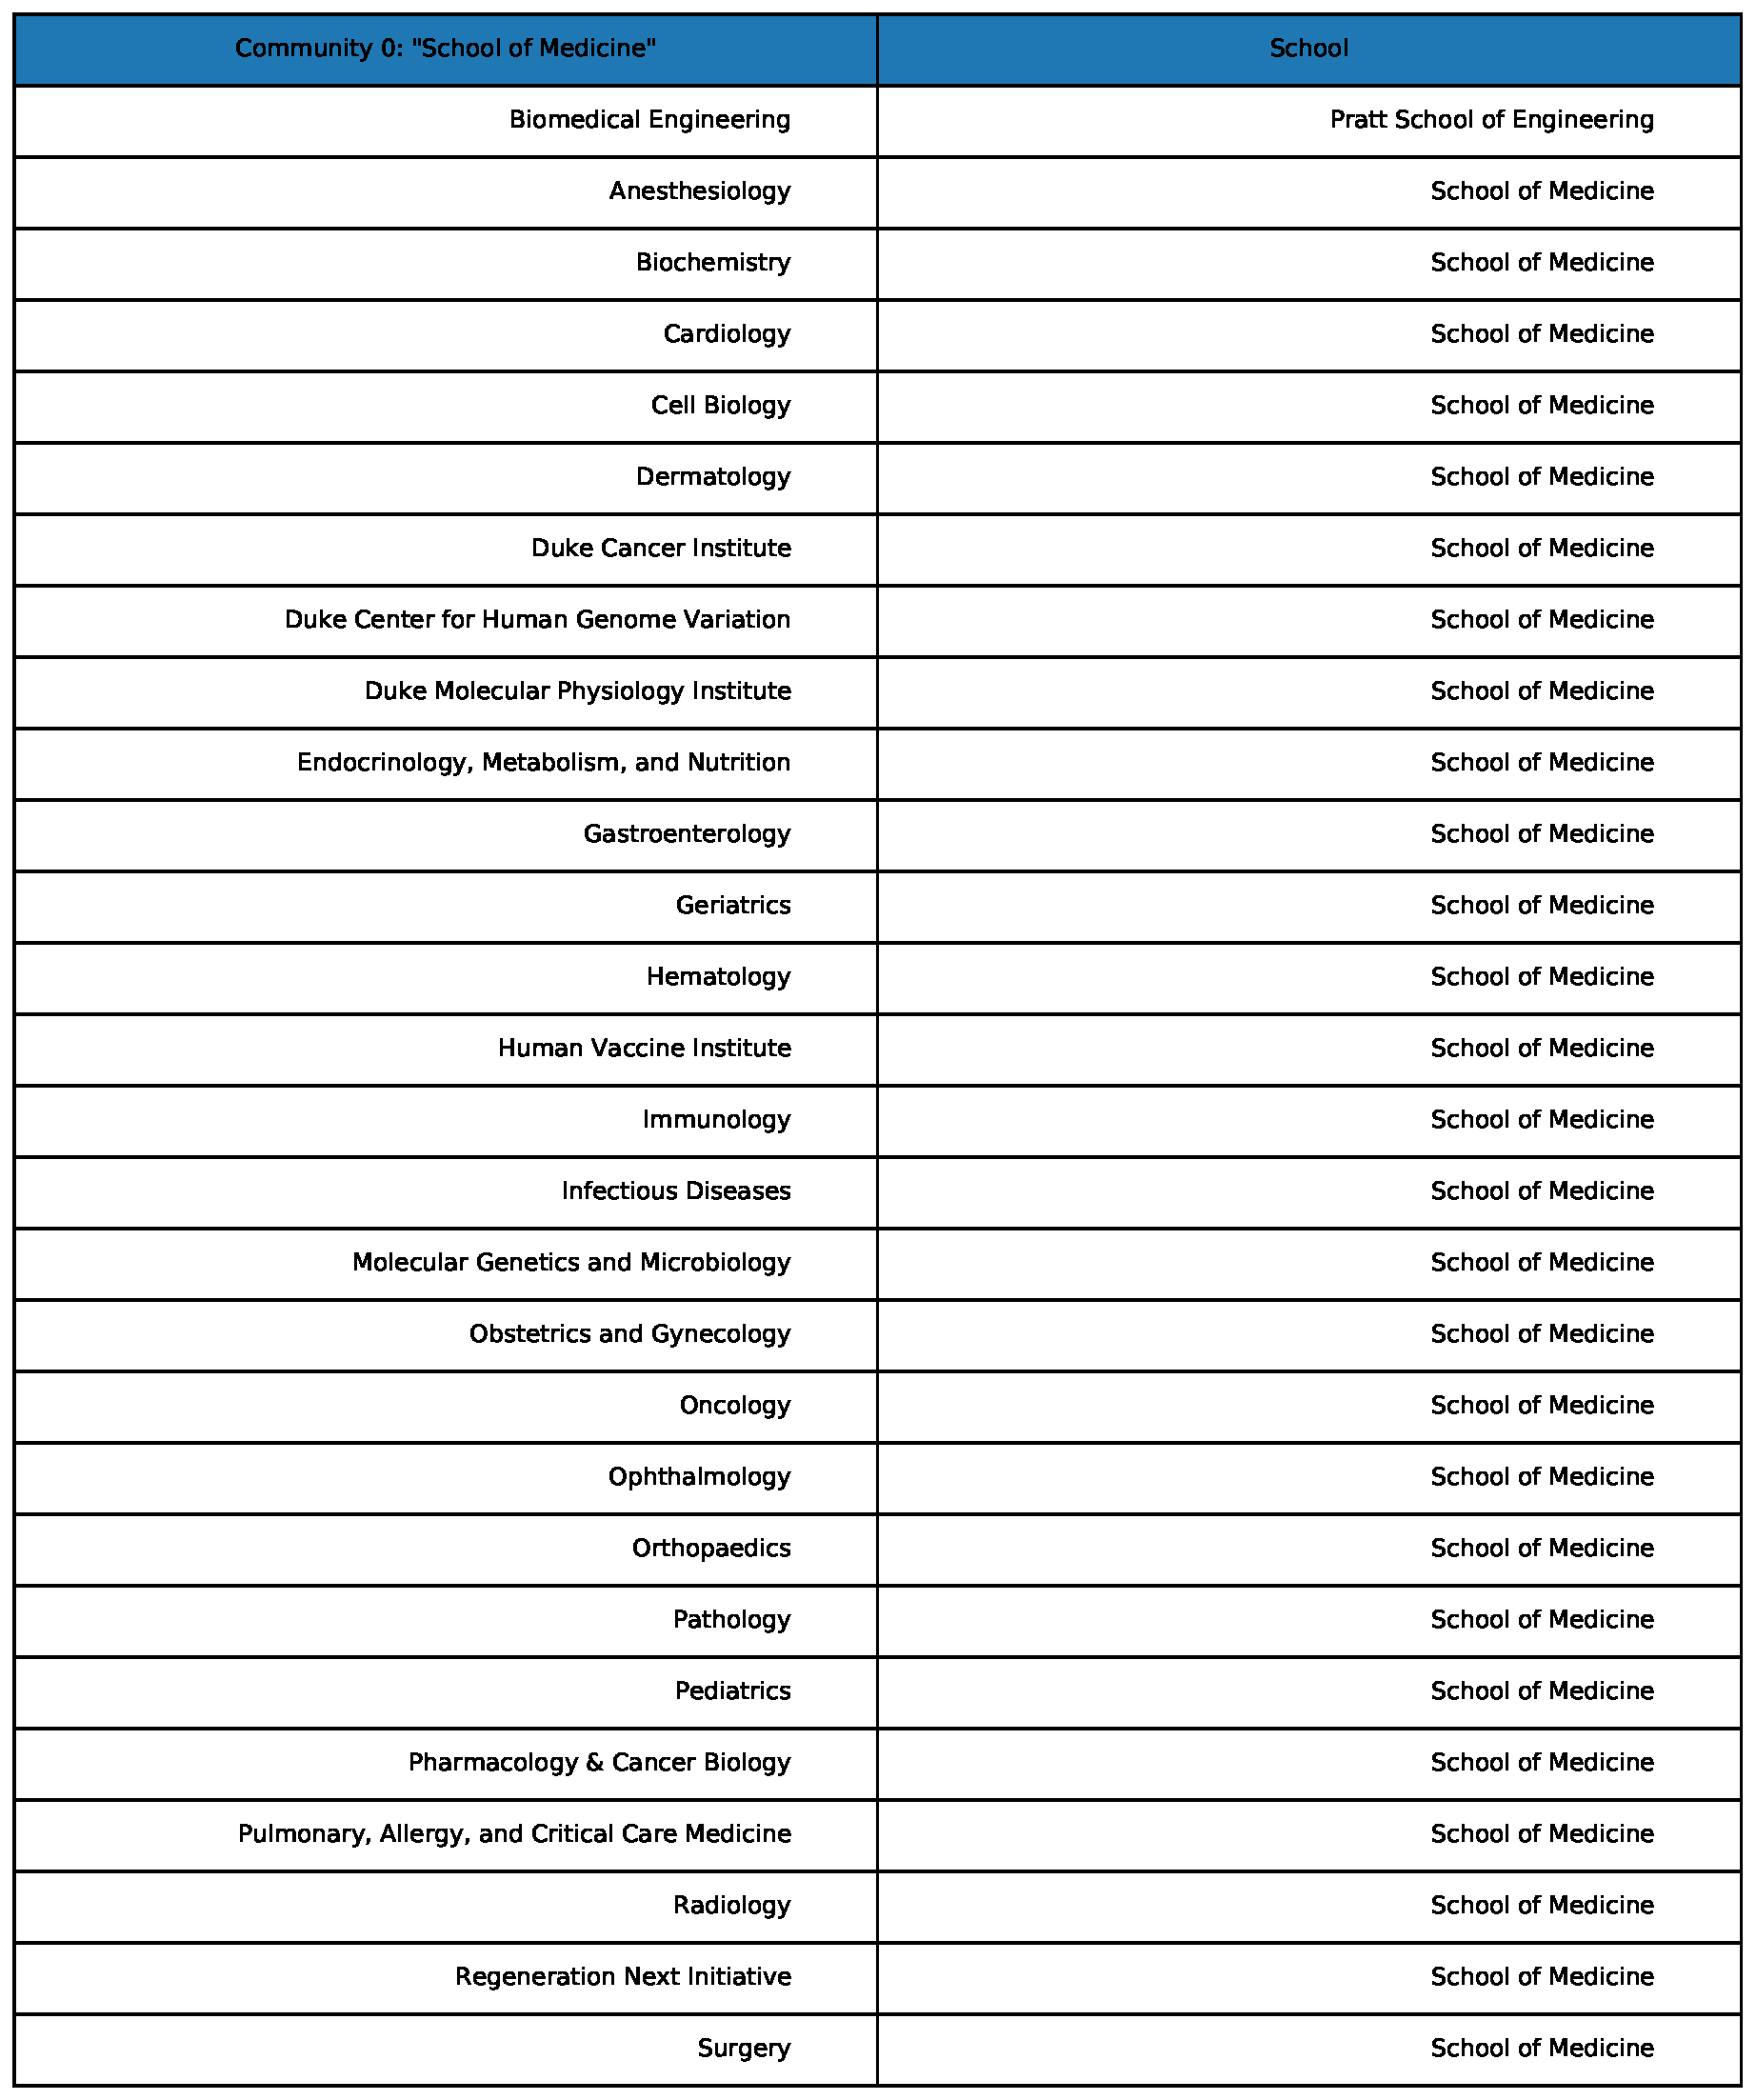
\includegraphics[width=\textwidth]{\figures/community_members/community_0_School_of_Medicine.pdf}
  \caption{Members of the ``School of Medicine" Louvain community.}
\end{figure}

\begin{figure}[!htb]\centering
  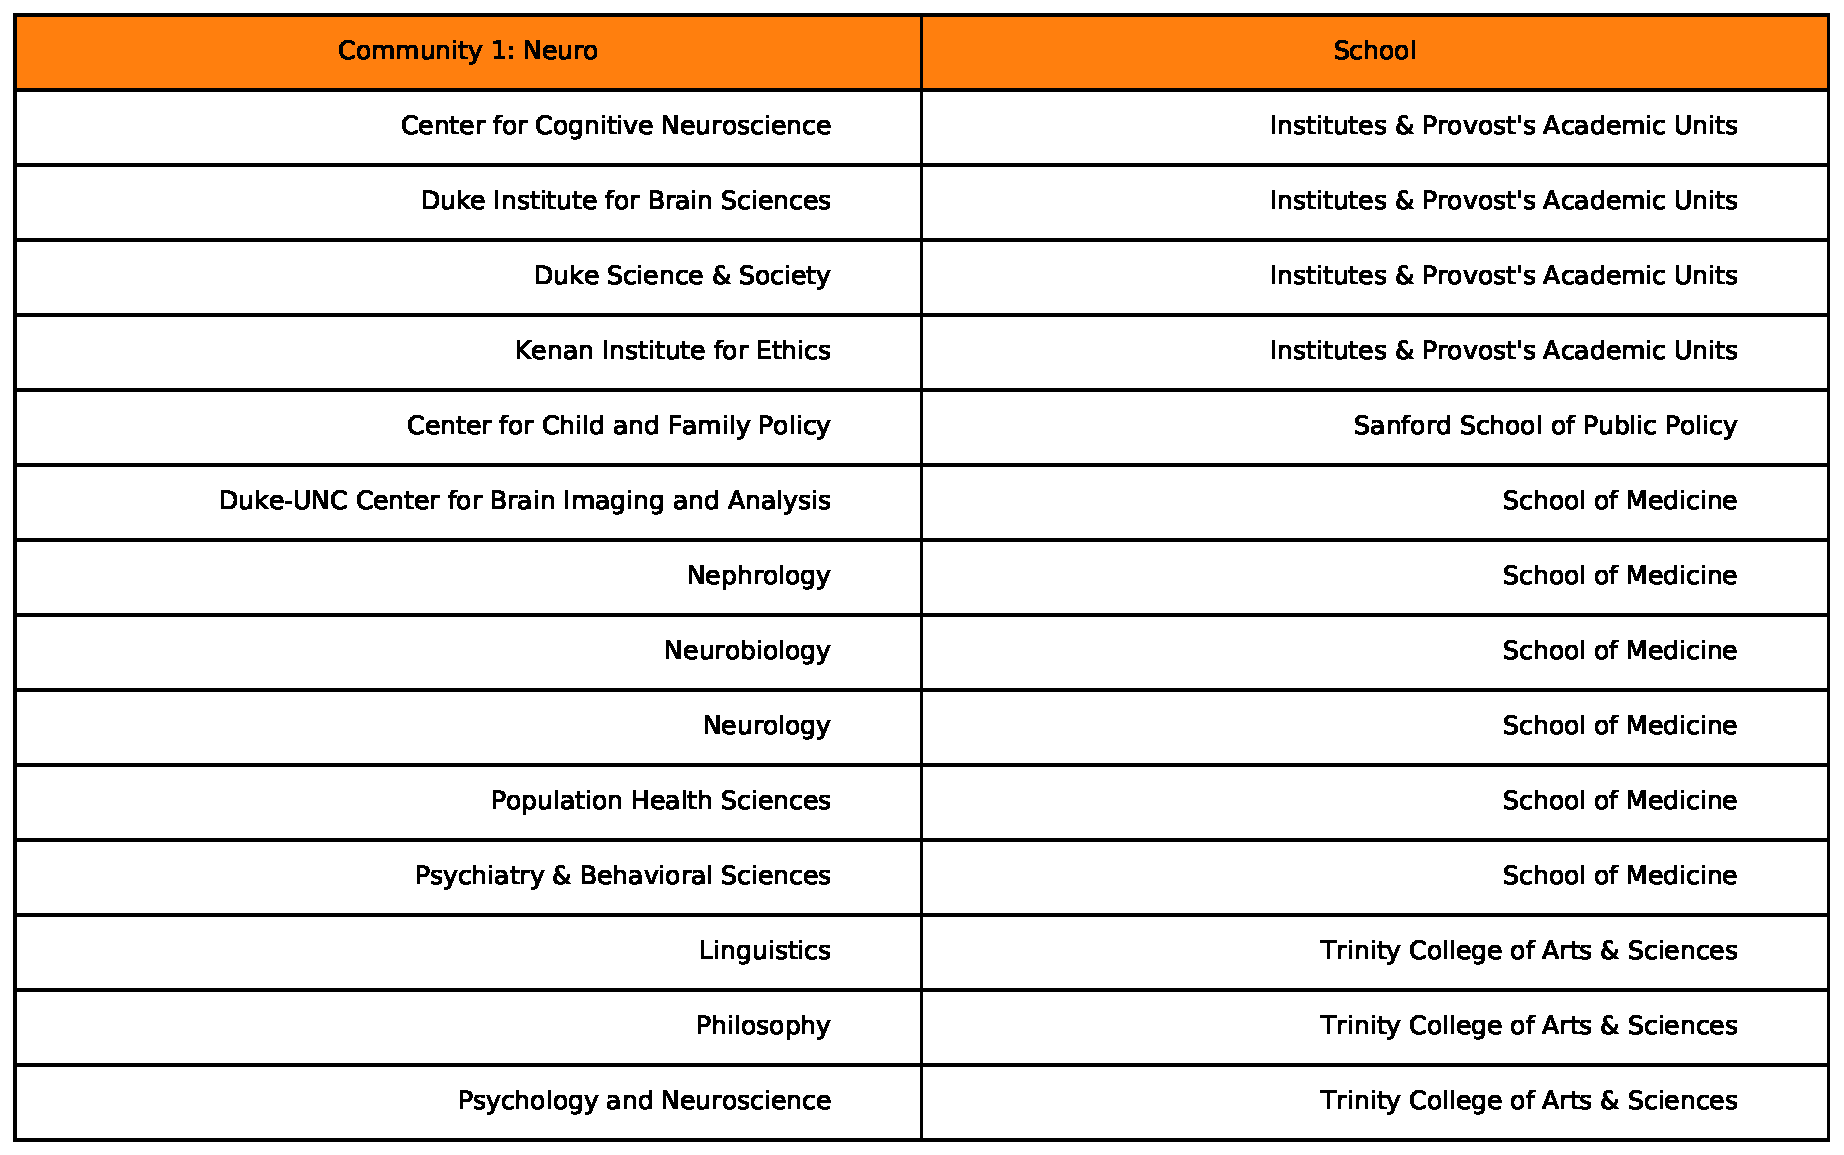
\includegraphics[width=\textwidth]{\figures/community_members/community_1_Neuro.pdf}
  \caption{Members of the Neuro Louvain community.}
\end{figure}

\begin{figure}[!htb]\centering
  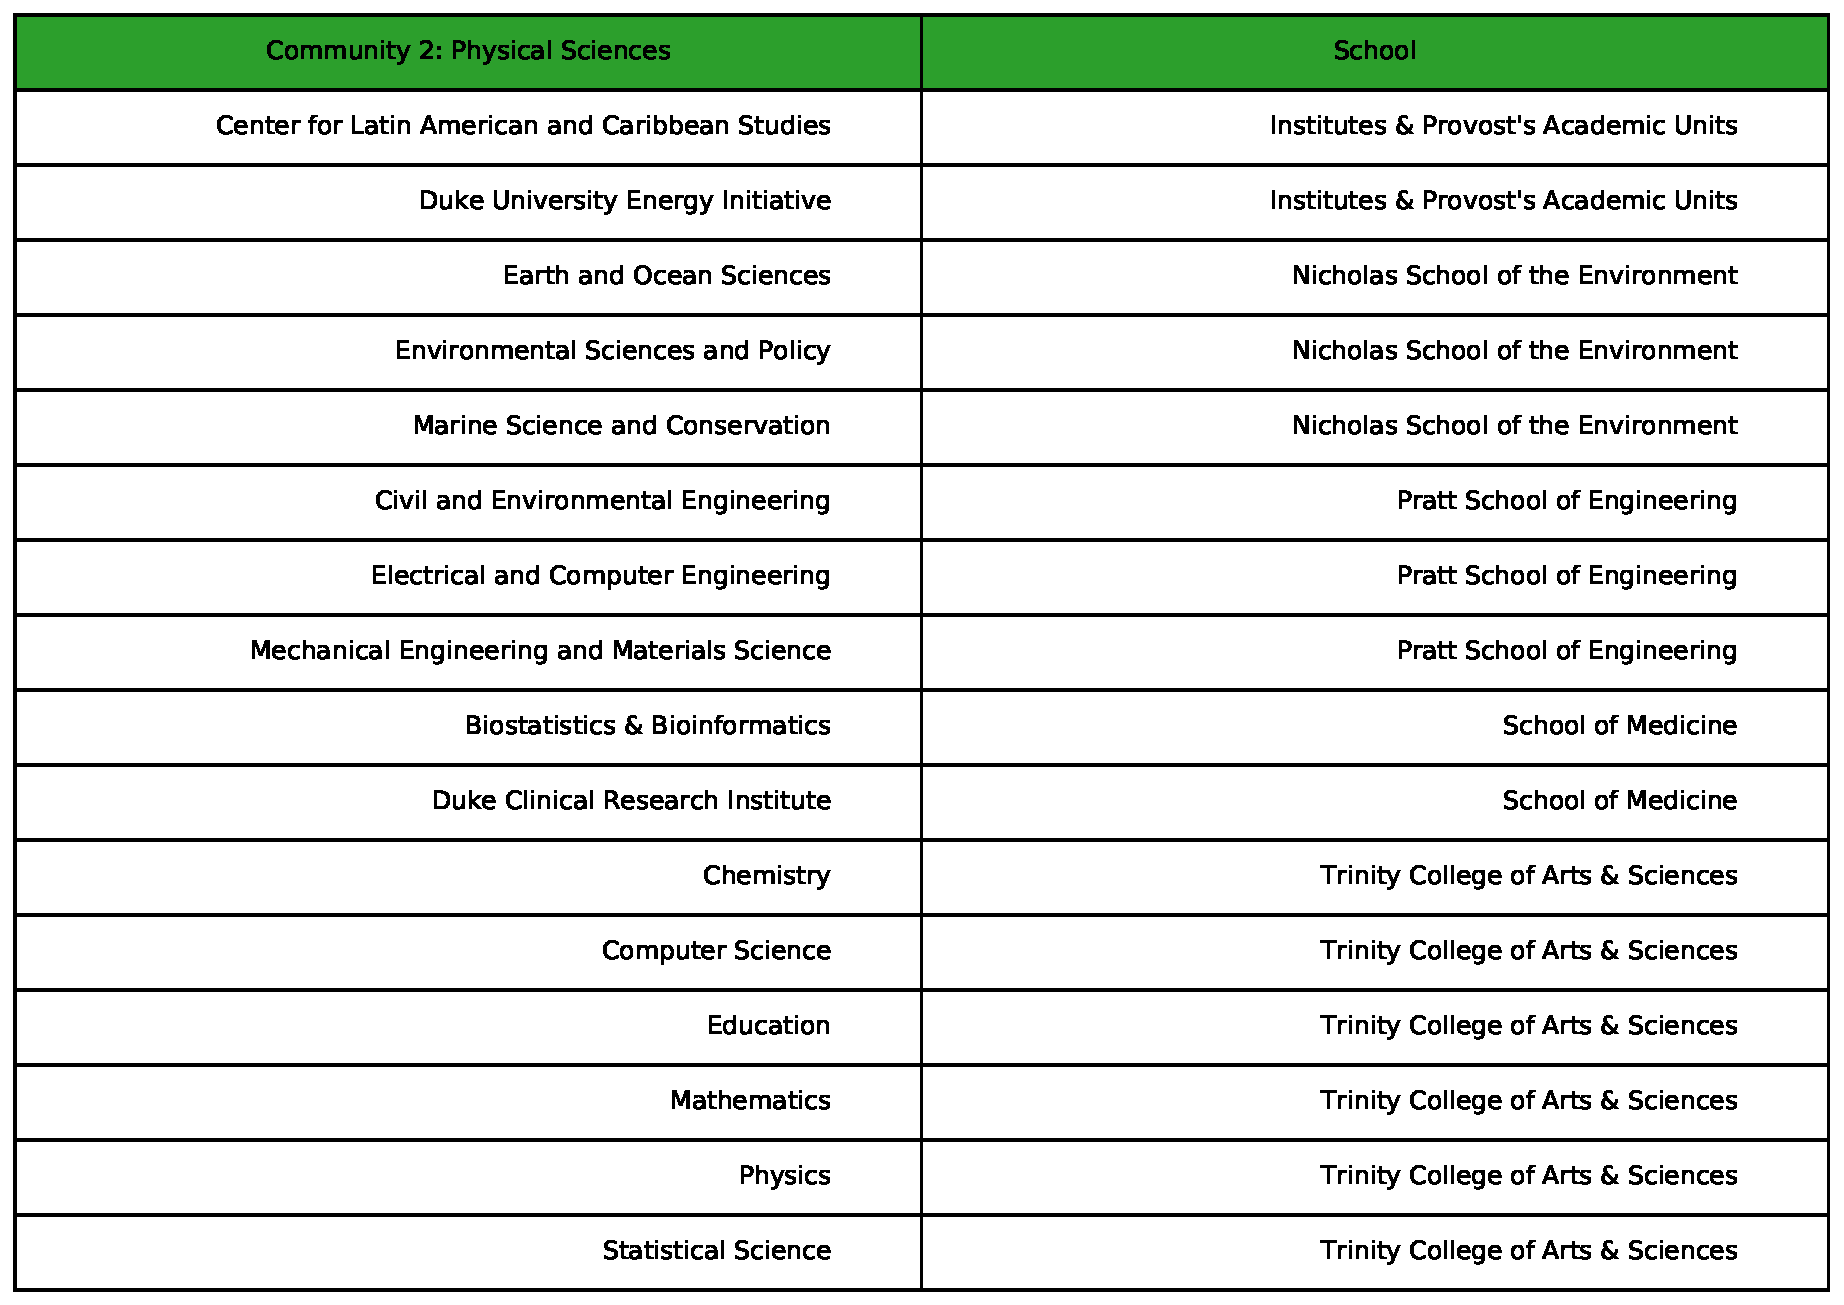
\includegraphics[width=\textwidth]{\figures/community_members/community_2_Physical_Sciences.pdf}
  \caption{Members of the Physical Sciences Louvain community.}
  \label{fig:f_community_physical_sciences}
\end{figure}

\begin{figure}[!htb]\centering
  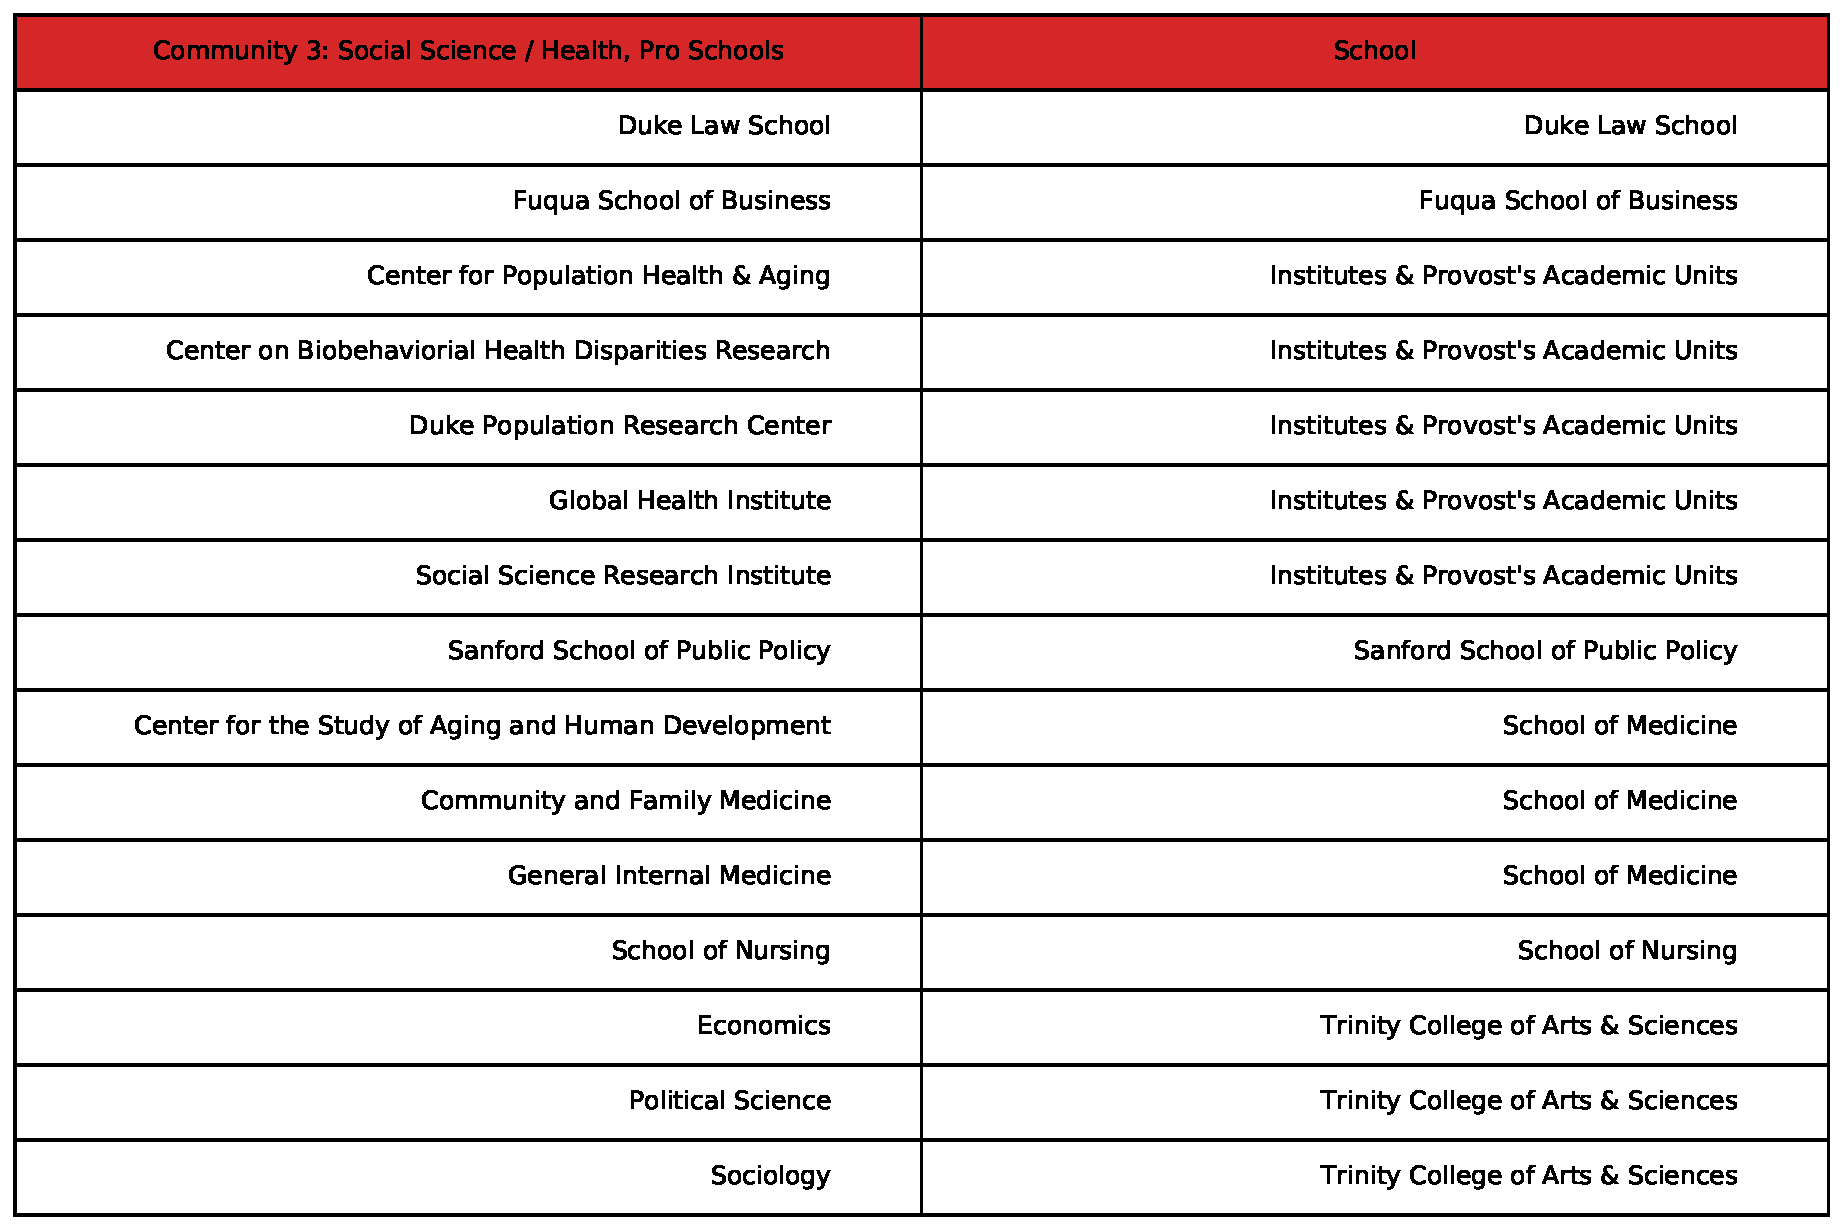
\includegraphics[width=\textwidth]{\figures/community_members/community_3_Social_Science_slash_Health_Pro_Schools.pdf}
  \caption{Members of the Social Science / Health, Pro Schools Louvain community.}
\end{figure}

\begin{figure}[!htb]\centering
  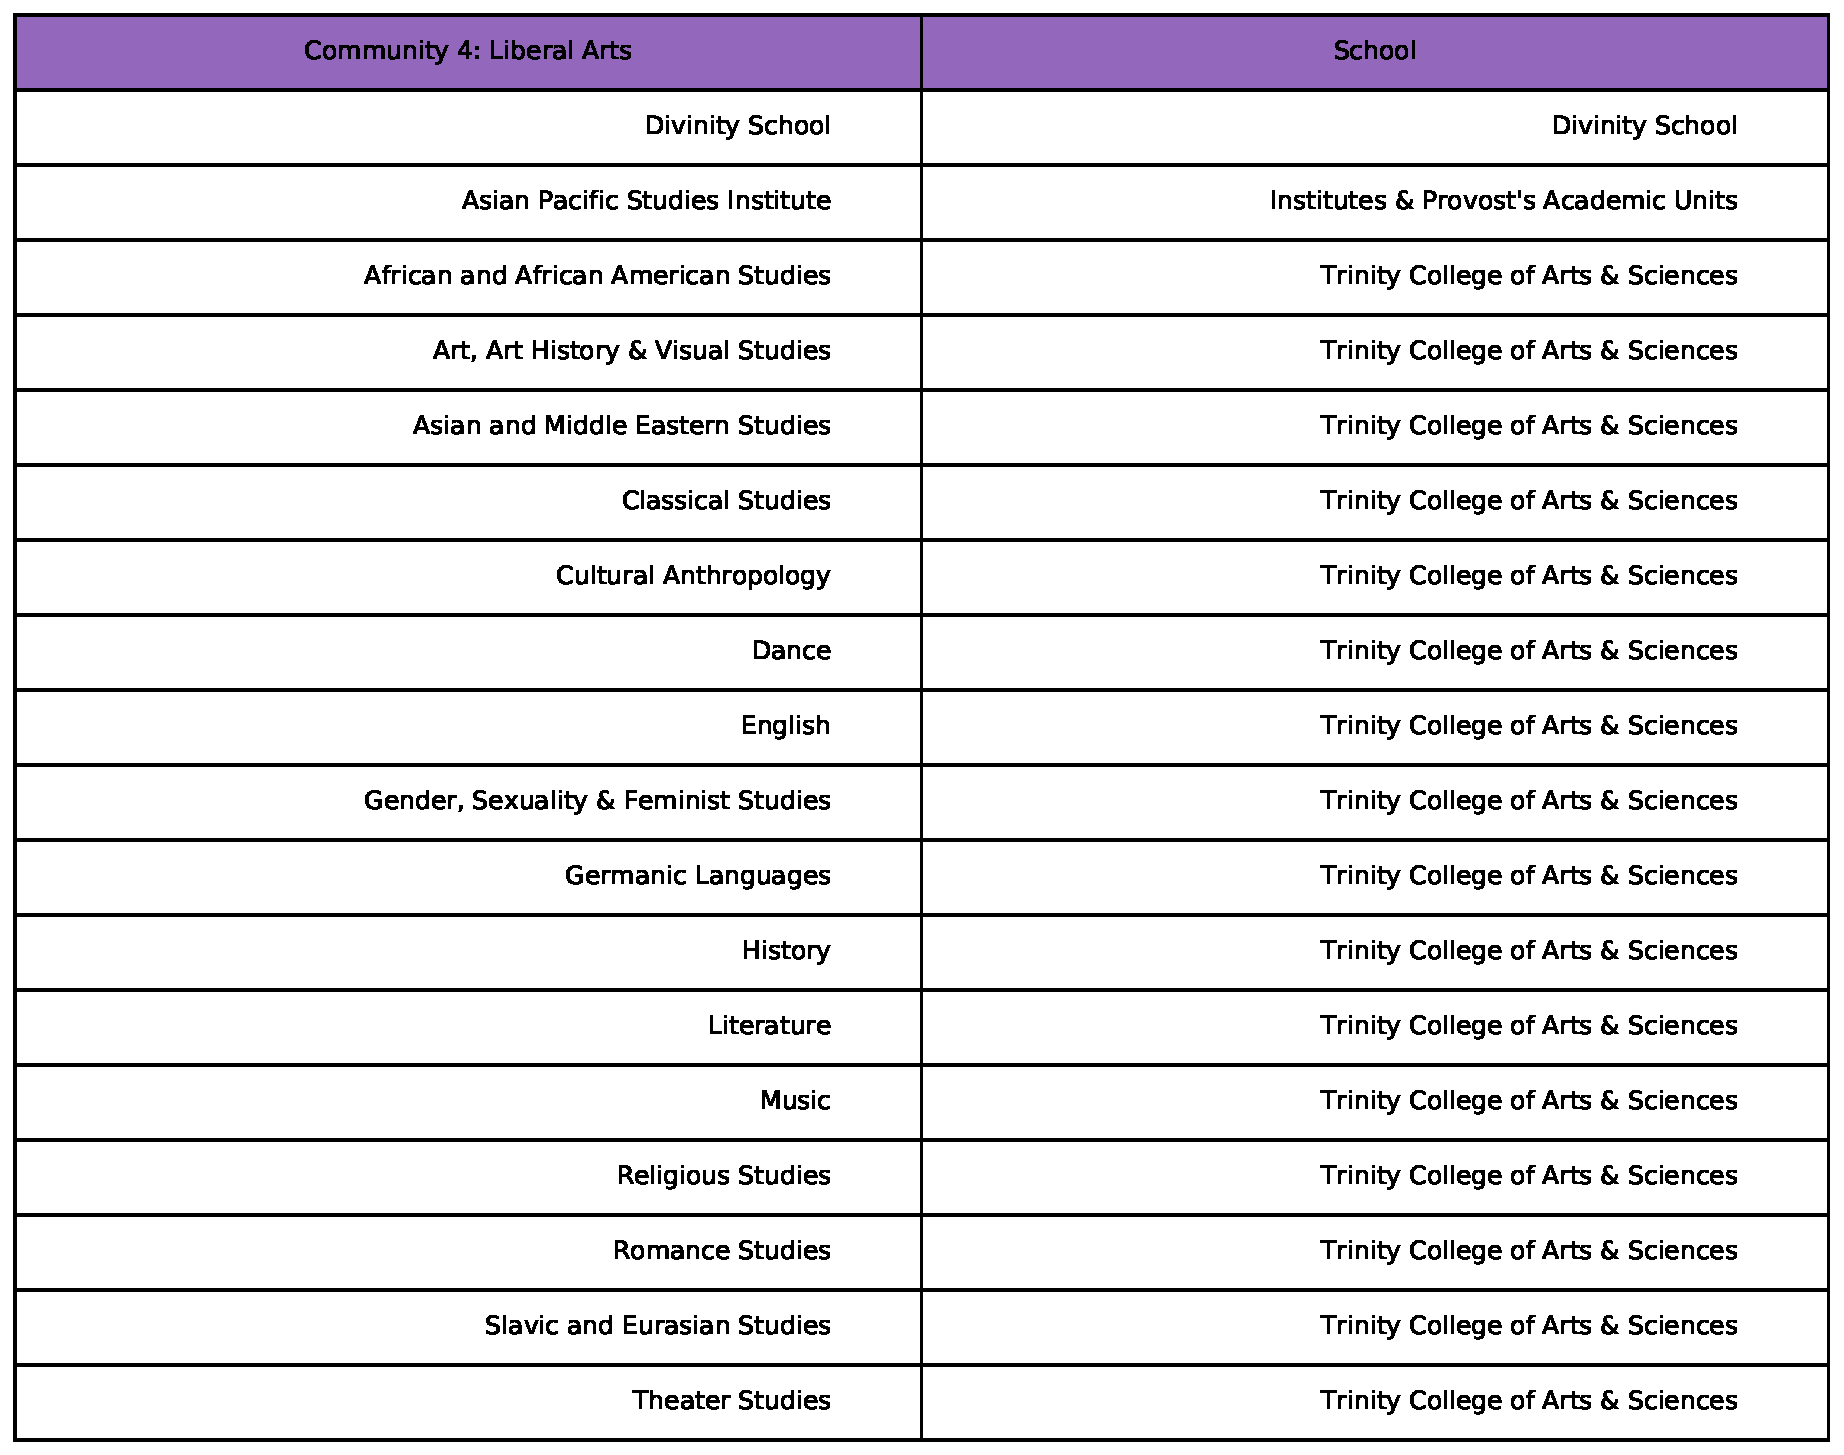
\includegraphics[width=\textwidth]{\figures/community_members/community_4_Liberal_Arts.pdf}
  \caption{Members of the Liberal Arts Louvain community.}
\end{figure}

\begin{figure}[!htb]\centering
  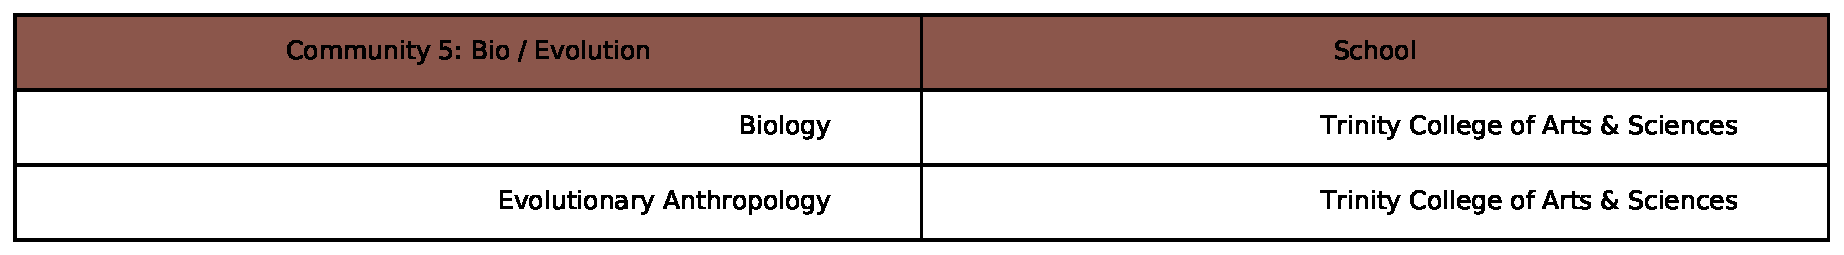
\includegraphics[width=\textwidth]{\figures/community_members/community_5_Bio_slash_Evolution.pdf}
  \caption{Members of the Bio / Evolution Louvain community.}
\end{figure}


\section{Interdisciplinary Fraction by Community}
\label{appendix:interdis_frac_community}

\begin{figure}[!htb]\centering
  \includegraphics[width=\textwidth]{\figures/interdis_frac/communities/School_of_Medicine.pdf}
  \caption{Interdisciplinary fraction vs year for the ``School of Medicine'' community.}
\end{figure}

\begin{figure}[!htb]\centering
  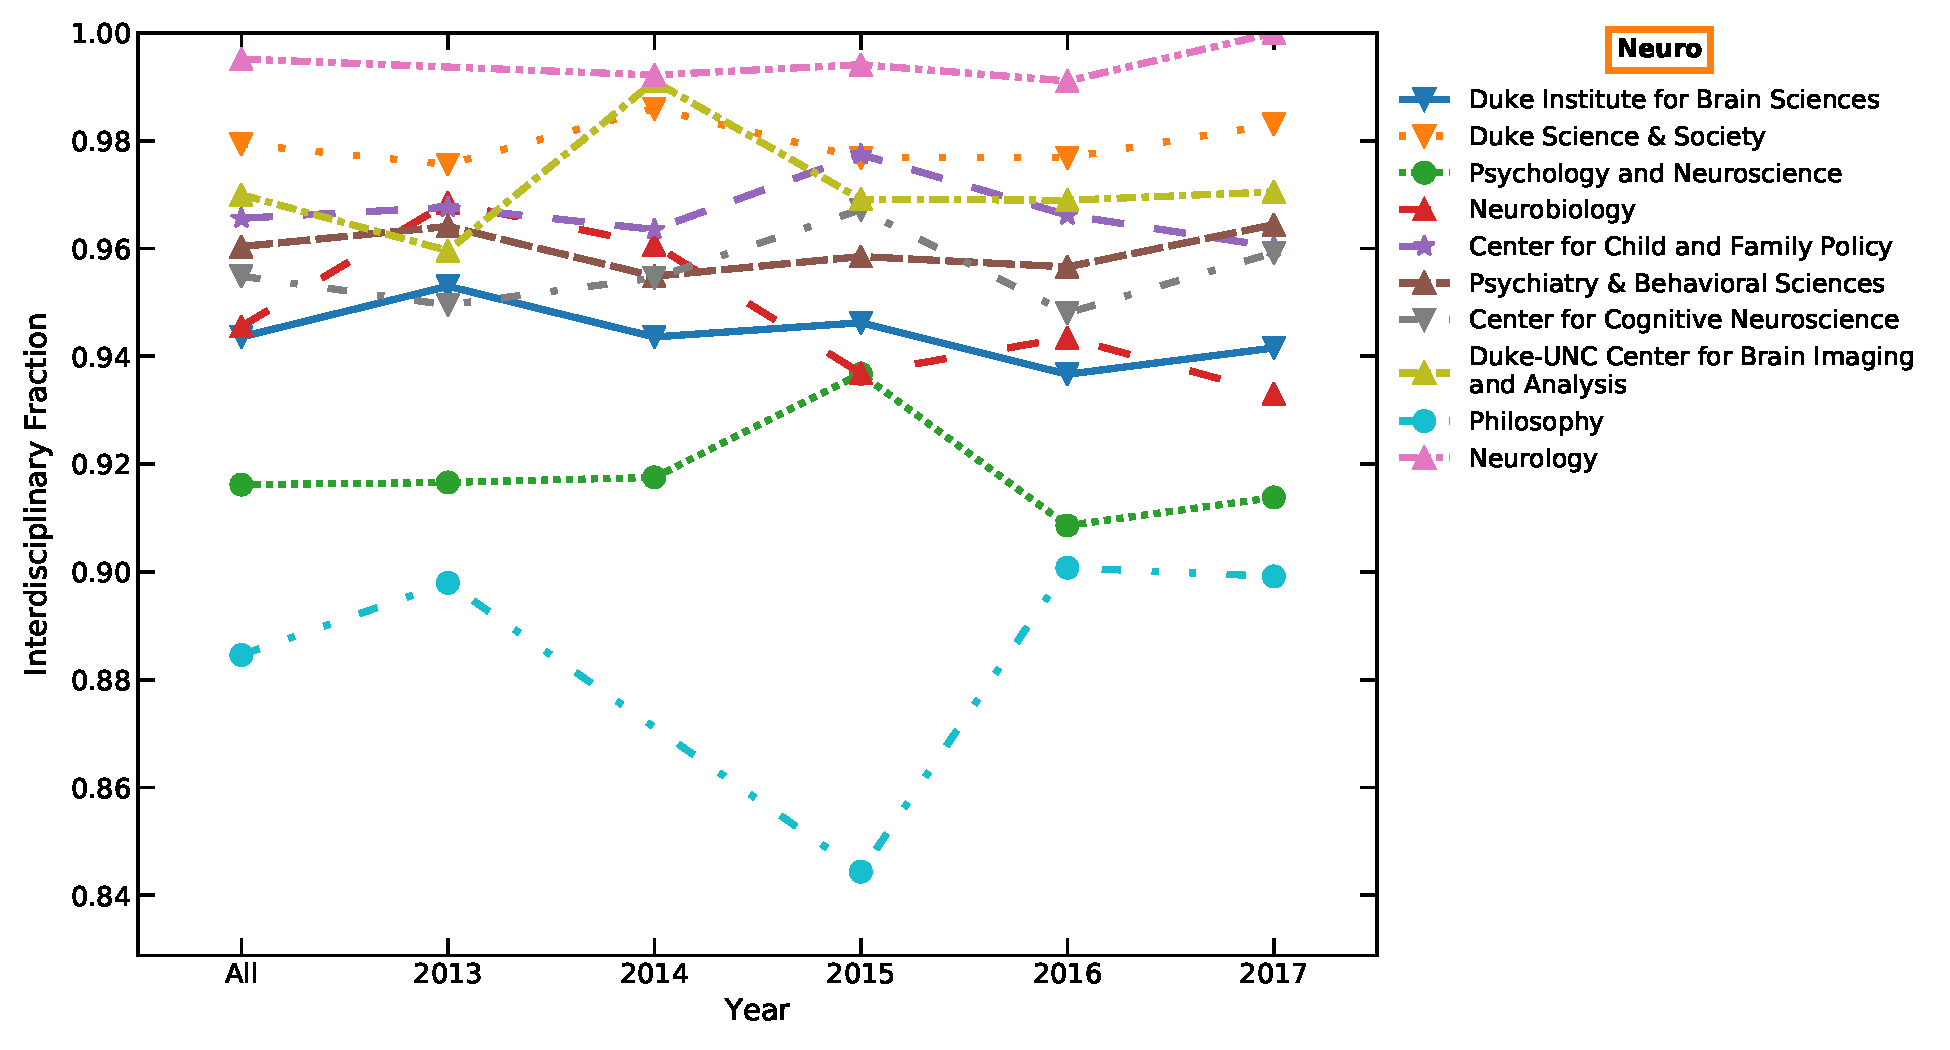
\includegraphics[width=\textwidth]{\figures/interdis_frac/communities/Neuro.pdf}
  \caption{Interdisciplinary fraction vs year for the Neuro community. Figure~\ref{fig:interdis_frac_neuro} reproduced for convenience.}
\end{figure}

\begin{figure}[!htb]\centering
  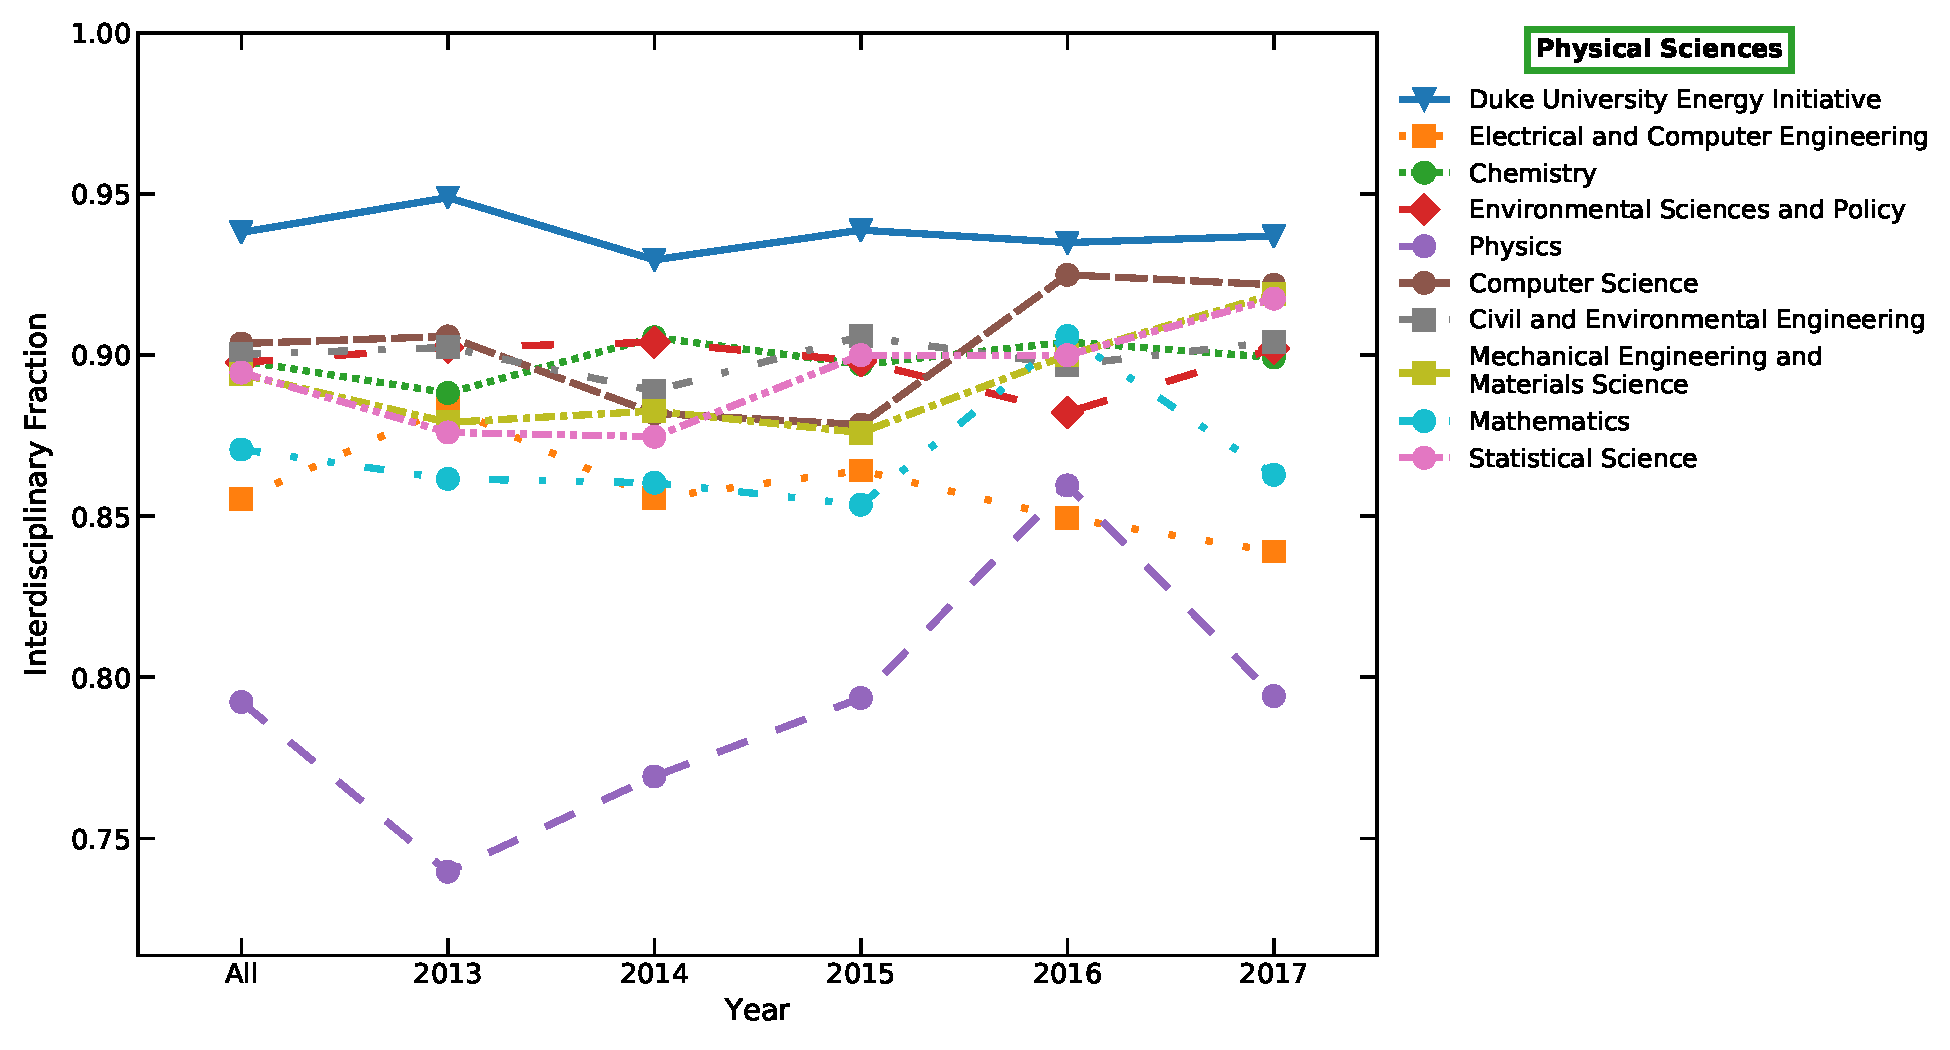
\includegraphics[width=\textwidth]{\figures/interdis_frac/communities/Physical_Sciences.pdf}
  \caption{Interdisciplinary fraction vs year for the Physical Sciences community. Figure~\ref{fig:interdis_frac_physical_sciences} reproduced for convenience.}
\end{figure}

\begin{figure}[!htb]\centering
  \includegraphics[width=\textwidth]{\figures/interdis_frac/communities/Social_Science_slash_Health,_Pro_Schools.pdf}
  \caption{Interdisciplinary fraction vs year for the Social Science / Health, Pro Schools community.}
\end{figure}

\begin{figure}[!htb]\centering
  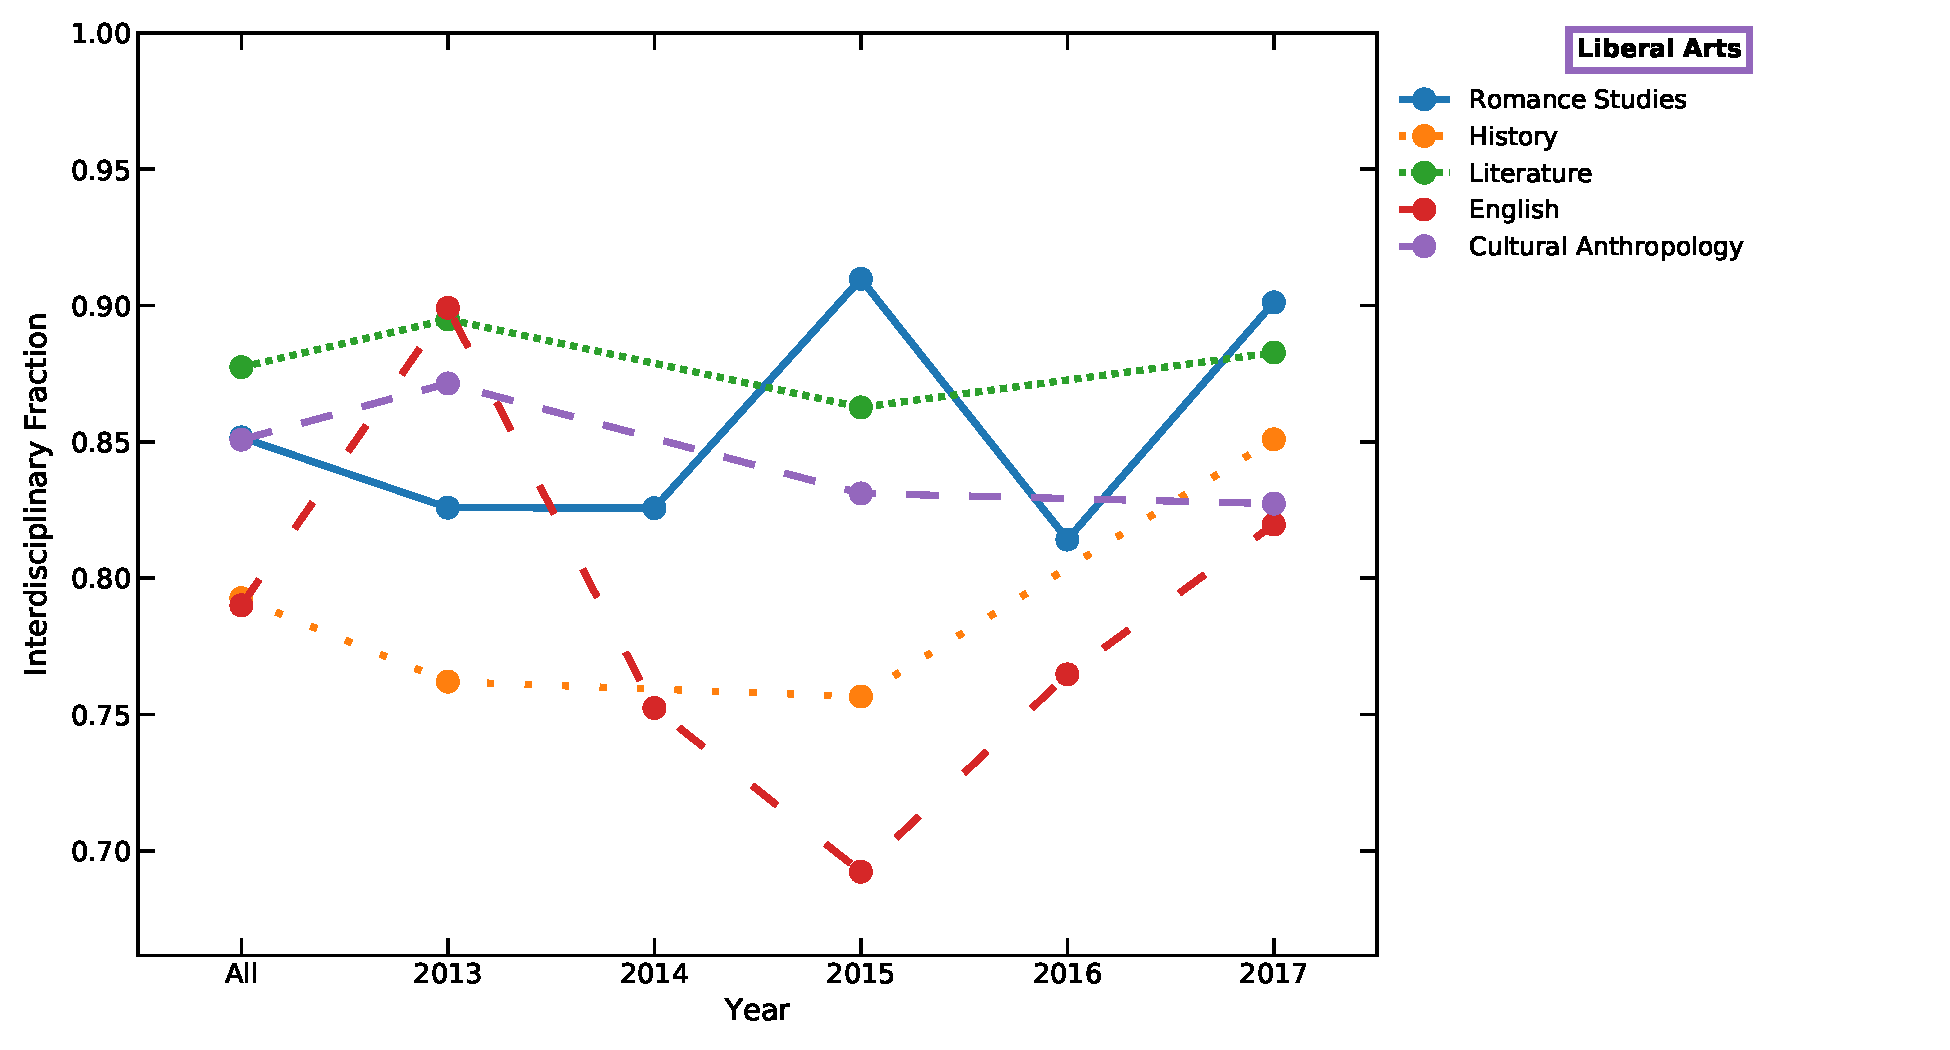
\includegraphics[width=\textwidth]{\figures/interdis_frac/communities/Liberal_Arts.pdf}
  \caption{Interdisciplinary fraction vs year for the Liberal Arts community. Figure~\ref{fig:interdis_frac_liberal_arts} reproduced for convenience.}
\end{figure}

\begin{figure}[!htb]\centering
  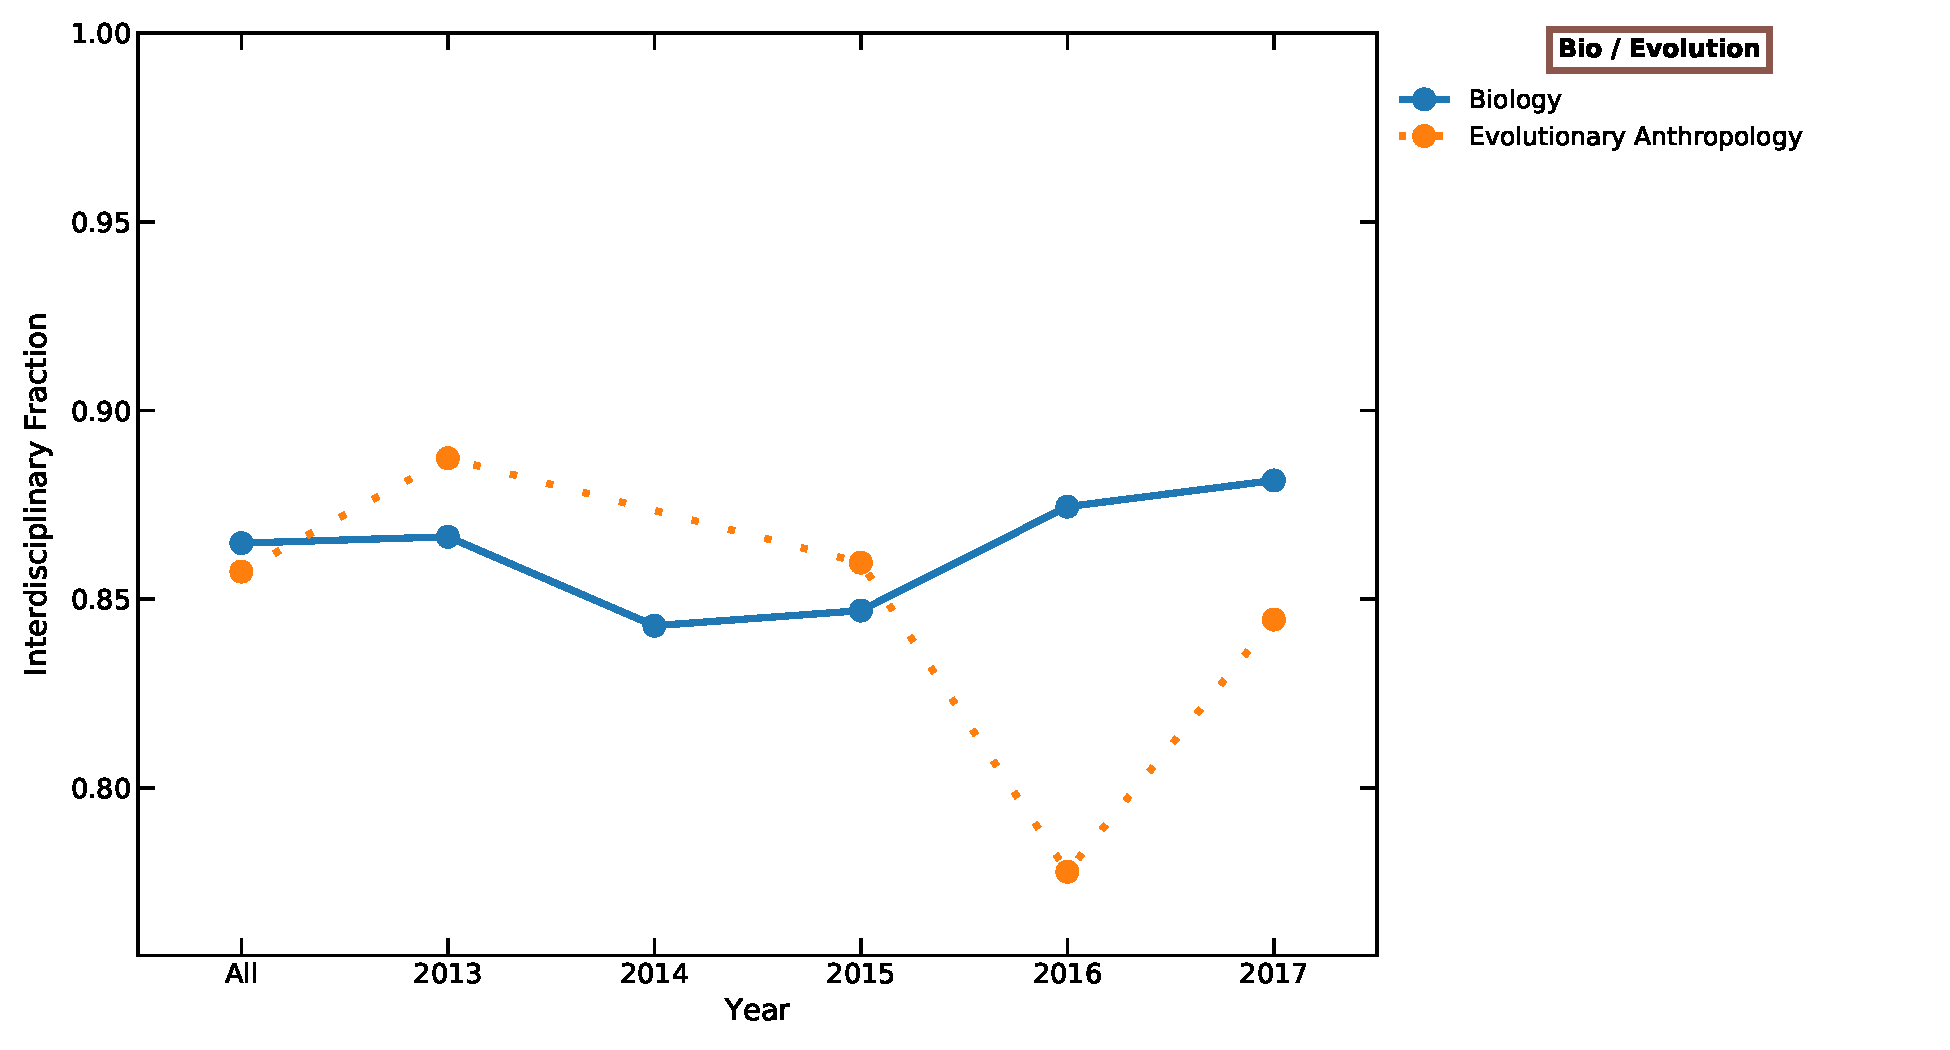
\includegraphics[width=\textwidth]{\figures/interdis_frac/communities/Bio_slash_Evolution.pdf}
  \caption{Interdisciplinary fraction vs year for the Bio / Evolution community.}
\end{figure}


\section{Interdisciplinary Fraction by School}
\label{appendix:interdis_frac_school}

\begin{figure}[!htb]\centering
  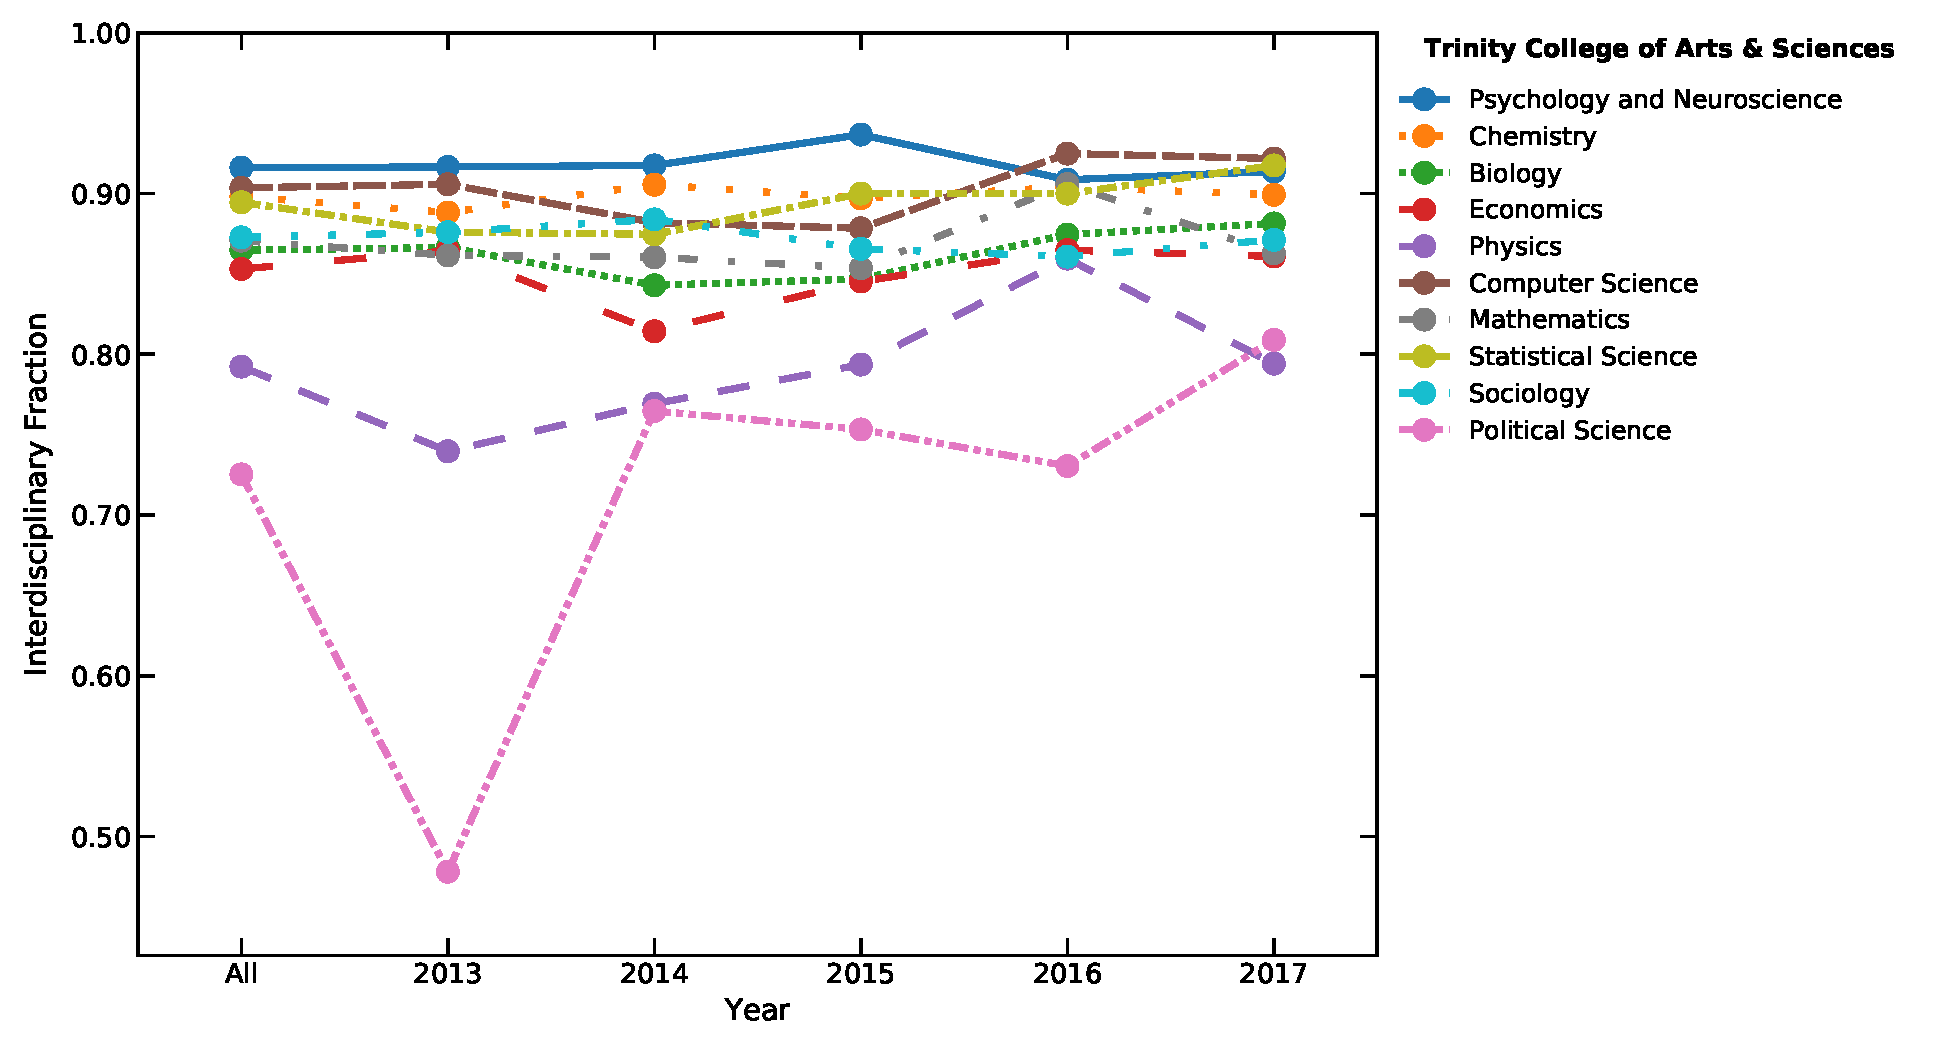
\includegraphics[width=\textwidth]{\figures/interdis_frac/schools/Trinity_College_of_Arts_and_Sciences.pdf}
  \caption{Interdisciplinary fraction vs year for the Trinity College of Arts \& Sciences.}
\end{figure}

\begin{figure}[!htb]\centering
  \includegraphics[width=\textwidth]{\figures/interdis_frac/schools/School_of_Medicine.pdf}
  \caption{Interdisciplinary fraction vs year for the School of Medicine.}
\end{figure}

\begin{figure}[!htb]\centering
  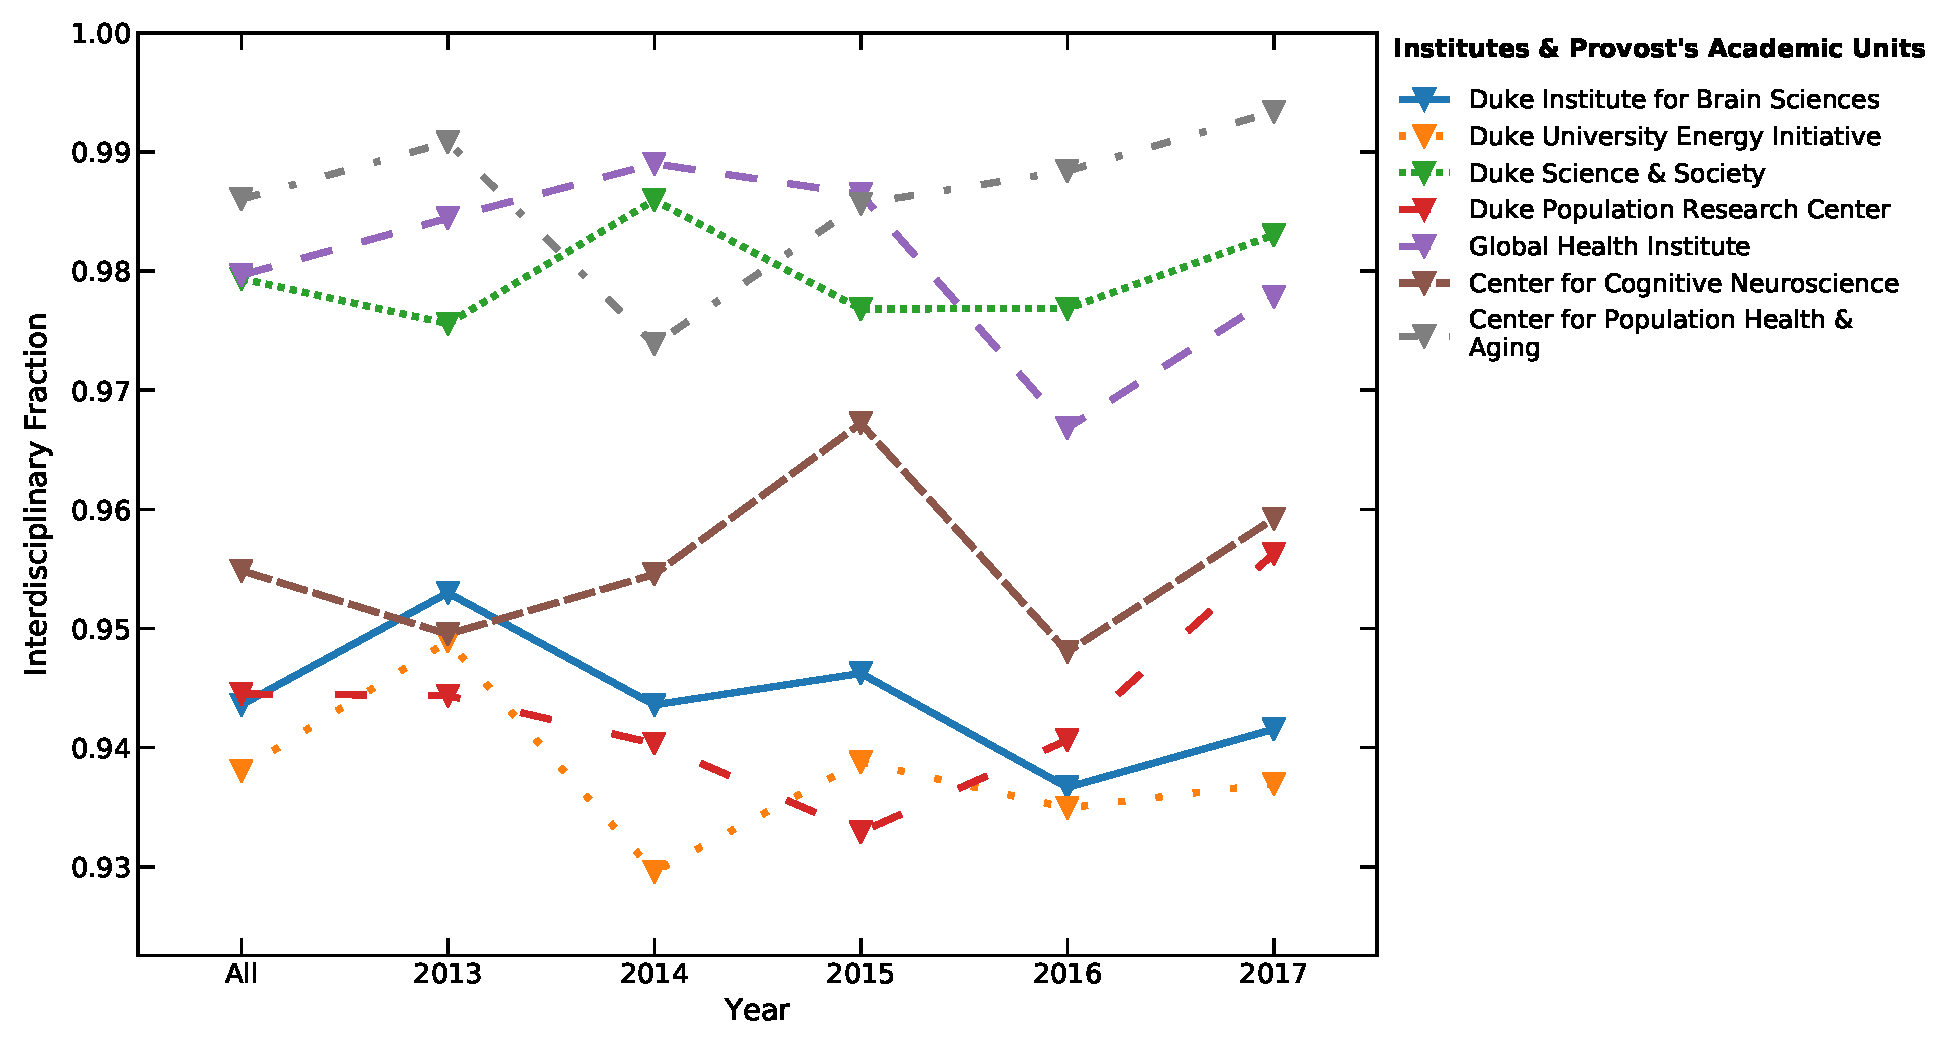
\includegraphics[width=\textwidth]{\figures/interdis_frac/schools/Institutes_and_Provosts_Academic_Units.pdf}
  \caption{Interdisciplinary fraction vs year for the Institutes \& Provost's Academic Units.}
\end{figure}

\begin{figure}[!htb]\centering
  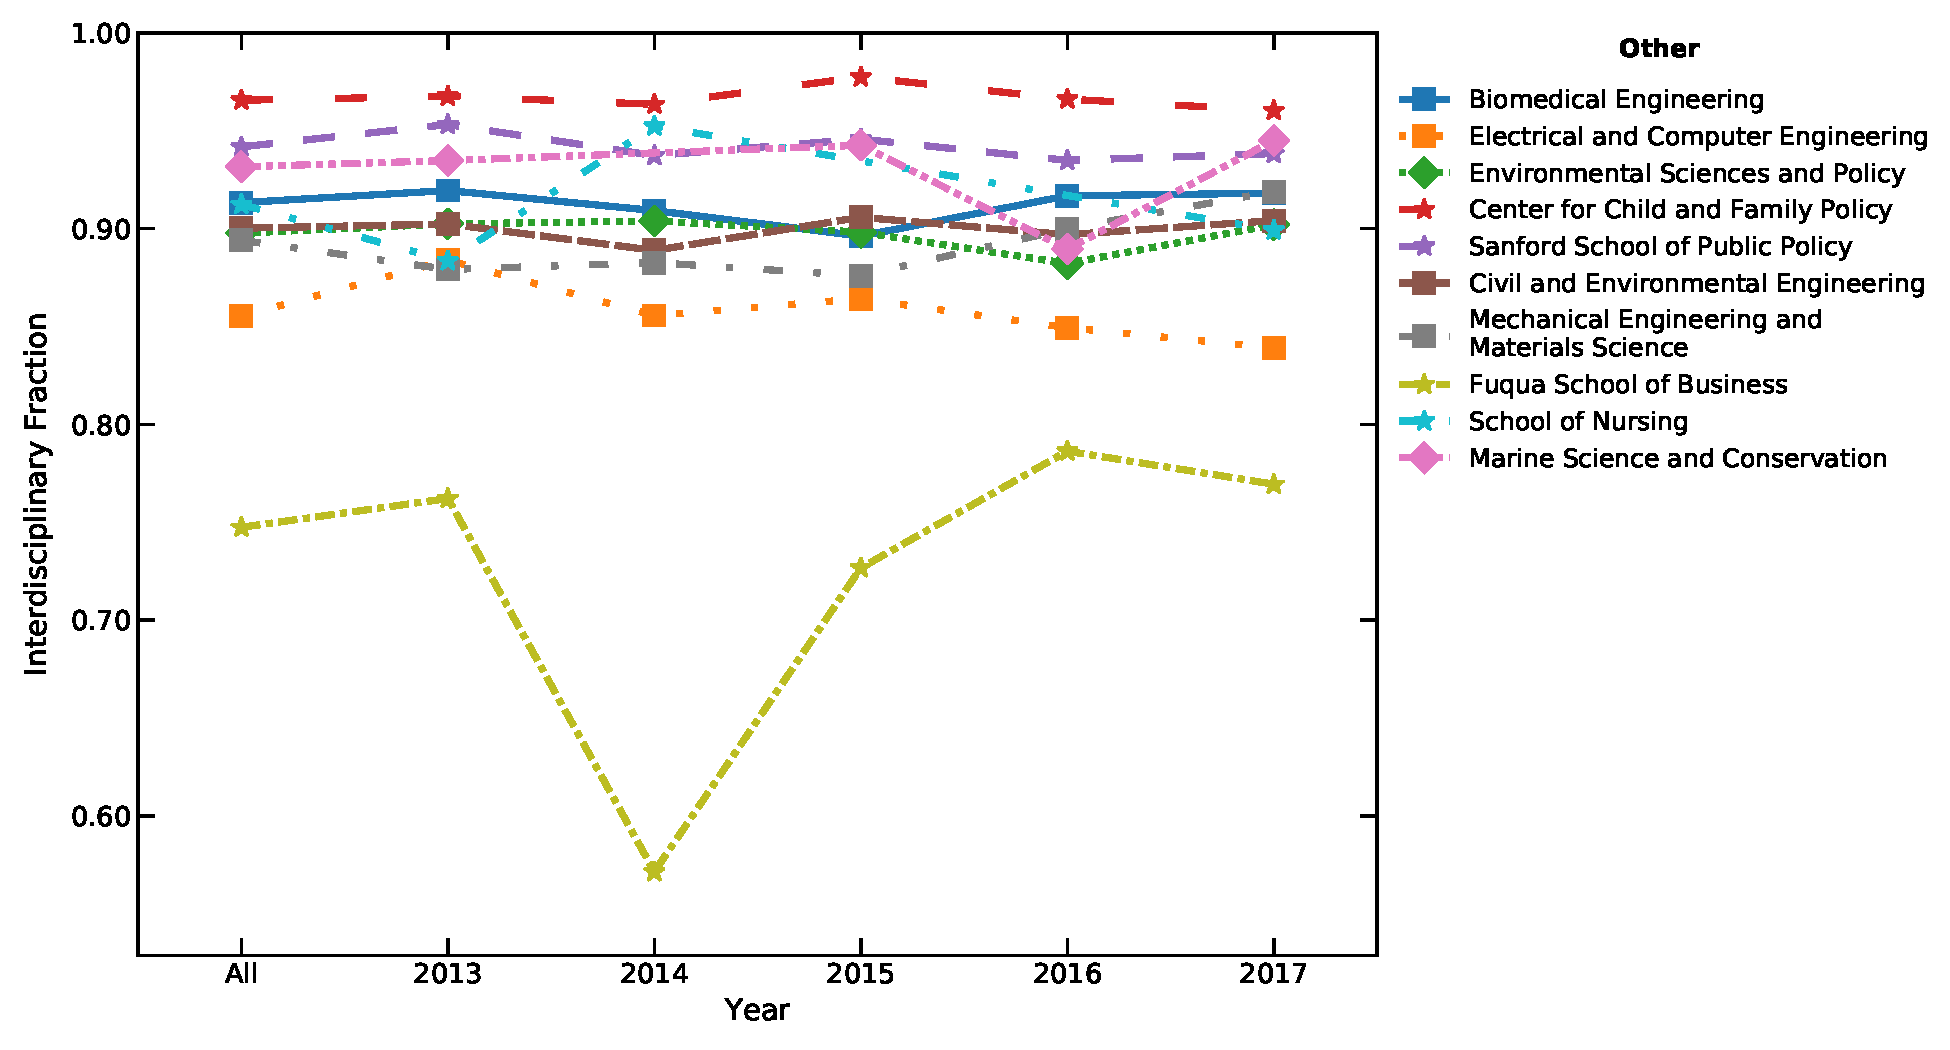
\includegraphics[width=\textwidth]{\figures/interdis_frac/schools/Other.pdf}
  \caption{Interdisciplinary fraction vs year for the remaining schools and units.}
\end{figure}

\end{appendices}

\end{document}
